% =============================================================================
% AIN-3009 — MLOps Term Project (Final Report)
% Compile from the `reports/` directory: pdflatex final_report.tex (twice)
% =============================================================================
\documentclass[11pt,a4paper]{article}

\usepackage[utf8]{inputenc}
\usepackage[T1]{fontenc}
\usepackage{lmodern}
\usepackage[english]{babel}

\usepackage[margin=2.5cm]{geometry}
\usepackage{setspace}
\setstretch{1.15}
\usepackage{microtype}
\usepackage{parskip}

\usepackage{graphicx}
\usepackage{url}
\graphicspath{{figures/}{screenshots/}}
\usepackage{booktabs}
\usepackage{array}
\usepackage{tabularx}
\usepackage{longtable}
\usepackage{caption}
\usepackage{subcaption}
\captionsetup{font=small,labelfont=bf}
\usepackage{float}

\usepackage{xcolor}
\definecolor{codebg}{HTML}{F6F8FA}
\definecolor{codekey}{HTML}{1F4E79}
\definecolor{coderule}{HTML}{D0D7DE}
\usepackage{listings}
\lstdefinestyle{shell}{
  basicstyle=\ttfamily\small,
  backgroundcolor=\color{codebg},
  frame=single,
  rulecolor=\color{coderule},
  framerule=0.4pt,
  breaklines=true,
  showstringspaces=false,
  columns=fullflexible,
  keepspaces=true,
}
\lstdefinestyle{json}{
  style=shell,
  language=,
  literate={\{}{{\textcolor{codekey}{\{}}}1
           {\}}{{\textcolor{codekey}{\}}}}1,
}

\usepackage{amsmath,amssymb}
\usepackage{fancyhdr}
\usepackage[hidelinks]{hyperref}

\hypersetup{
  pdftitle={Development and Evaluation of ML Lifecycle Management using MLflow},
  pdfauthor={Khaireddine Arbouch},
  pdfsubject={AIN-3009 MLOps Term Project},
  pdfkeywords={MLOps, MLflow, Machine Learning, Logistics, Delay Prediction}
}

% --- Header / footer ---
\pagestyle{fancy}
\fancyhf{}
\lhead{\small AIN-3009 — MLOps Term Project}
\rhead{\small K.\ Arbouch — 2281524}
\cfoot{\thepage}
\renewcommand{\headrulewidth}{0.4pt}

% --- Title metadata ---
\newcommand{\Course}{AIN-3009 — Development and Evaluation of ML Lifecycle Management}
\newcommand{\Assignment}{Term Project}
\newcommand{\AuthorName}{Khaireddine Arbouch}
\newcommand{\StudentID}{2281524}

\title{\vspace{-0.8cm}\textbf{Development and Evaluation of a Machine Learning\\
Lifecycle Management System using MLflow}\\[8pt]
\large A Comprehensive MLOps Implementation for\\
Logistics Shipment Delay Risk Prediction}
\author{}
\date{\today}

\begin{document}

% --- Title page ---
\begin{center}
{\LARGE\bfseries Development and Evaluation of a\\[4pt]
Machine Learning Lifecycle Management System\\[4pt]
using MLflow}\\[12pt]
{\large\itshape A Comprehensive MLOps Implementation for\\
Logistics Shipment Delay Risk Prediction}\\[20pt]
\rule{\linewidth}{0.5pt}\\[12pt]
\begin{tabular}{@{}ll@{}}
\textbf{Course:}      & \Course \\
\textbf{Assignment:}  & \Assignment \\
\textbf{Student Name:}        & \AuthorName \\
\textbf{Student ID:}  & \StudentID \\
\textbf{Submission Date:}        & \today \\
\end{tabular}\\[12pt]
\rule{\linewidth}{0.5pt}
\end{center}
\thispagestyle{empty}
\vspace{15pt}

\begin{abstract}
\noindent
This report presents a comprehensive implementation of a machine learning operations (MLOps) system for predicting shipment delay risk in logistics networks. The system demonstrates the complete machine learning lifecycle using MLflow as the central platform for experiment tracking, model registry, deployment, and monitoring. We develop and evaluate three baseline classification models (Logistic Regression, Random Forest, and Gradient Boosting) on a structured synthetic dataset comprising 6,000 shipment records with 12 features encoding operational risk factors. Hyperparameter optimization is performed using Optuna with nested MLflow runs, achieving a cross-validated F1-score of 0.9255. The champion model (Logistic Regression, test F1-score: 0.9324) is registered in the MLflow Model Registry, deployed via a FastAPI service, and monitored across five batch scenarios including four targeted drift conditions. The implementation achieves full reproducibility through deterministic data generation, comprehensive artifact logging, and automated deployment procedures. All experimental results are tracked and versioned through MLflow, demonstrating best practices in ML lifecycle management for operational intelligence applications.
\end{abstract}

\tableofcontents
\newpage

% =============================================================================
\section{Introduction}
\label{sec:intro}

\subsection{Background and Motivation}

Logistics networks face persistent challenges in maintaining on-time delivery performance due to complex interdependencies among operational factors including route characteristics, carrier capabilities, customs procedures, weather conditions, and port congestion. Shipment delays impose significant costs through contractual penalties, inventory holding expenses, and downstream supply chain disruptions. The ability to predict delay risk from structured shipment attributes represents a valuable operational intelligence capability for proactive resource allocation and customer communication.

\subsubsection{Business Value and Impact}

Predictive delay risk models deliver tangible business value across multiple dimensions:

\paragraph{Cost Reduction.}
Reducing shipment delays by even 5-10\% can significantly lower operational costs. Late deliveries trigger contractual penalties (typically 2-5\% of shipment value), expedited shipping costs to recover schedules, and increased inventory holding costs due to safety stock buffers. For a mid-sized logistics provider handling 10,000 shipments monthly with average value \$50,000, a 5\% reduction in delays could save \$2.5-5M annually in penalty avoidance alone.

\paragraph{Customer Satisfaction.}
Proactive delay prediction enables early customer notification, allowing downstream supply chain partners to adjust production schedules, inventory planning, and resource allocation. Studies show that proactive communication about delays improves customer satisfaction scores by 15-20\% compared to reactive notification after delays occur.

\paragraph{Operational Efficiency.}
Delay risk scores enable dynamic resource allocation: high-risk shipments can be prioritized for premium carriers, expedited customs clearance, or alternative routing. This targeted intervention is more cost-effective than blanket premium service upgrades.

\paragraph{Strategic Planning.}
Aggregated delay predictions inform strategic decisions about carrier partnerships, route optimization, and capacity planning. Identifying systematic delay patterns (e.g., specific origin-destination pairs, seasonal weather impacts) guides long-term network design.

\subsection{MLOps Challenges and Motivation}

Beyond the domain application, this project addresses a fundamental challenge in modern machine learning engineering: the gap between model development and operational deployment. Traditional machine learning workflows often lack systematic approaches to experiment tracking, model versioning, deployment automation, and performance monitoring. The emergence of Machine Learning Operations (MLOps) practices and platforms aims to bridge this gap by providing structured methodologies and tooling for the complete ML lifecycle.

\subsection{Project Objectives}

This project implements a comprehensive MLOps system demonstrating best practices across five critical lifecycle stages:

\begin{enumerate}
    \item \textbf{Experiment Tracking}: Systematic logging of model parameters, performance metrics, and artifacts across multiple training runs
    \item \textbf{Model Training and Tuning}: Development of baseline models and systematic hyperparameter optimization with full provenance tracking
    \item \textbf{Model Registry}: Version management and promotion workflows for production model selection
    \item \textbf{Model Deployment}: Automated serving infrastructure loading registered models without retraining
    \item \textbf{Performance Monitoring}: Continuous evaluation of model performance and data distribution shifts in production
\end{enumerate}

The implementation uses MLflow as the central platform, providing a unified interface for tracking, registry, and deployment operations. The system is designed for full reproducibility, with deterministic data generation, explicit random seeds, and comprehensive documentation of all experimental procedures.

\subsection{Scope and Limitations}

\paragraph{Data Provenance.}
The primary dataset is synthetically generated using a transparent probabilistic model with domain-motivated feature relationships. While this approach ensures reproducibility and interpretability of experimental results, the reported performance metrics should be understood as validation of pipeline correctness rather than claims of commercial accuracy on real logistics networks. The synthetic generation process is documented in Section~\ref{sec:data} and implemented with deterministic random seeds to ensure exact reproducibility.

\paragraph{Technical Scope.}
The implementation focuses on classical machine learning approaches (logistic regression, tree ensembles) rather than deep learning, prioritizing interpretability and computational efficiency appropriate for structured tabular data. Deployment is configured for local execution using SQLite backend storage and filesystem artifact management, though the architecture extends naturally to cloud-based MLflow deployments with minimal configuration changes.

\subsection{Contributions}

This work makes the following contributions to MLOps practice and pedagogy:

\begin{itemize}
    \item A complete, reproducible implementation of the MLflow lifecycle demonstrating integration of tracking, registry, serving, and monitoring components
    \item A structured approach to hyperparameter tuning with nested MLflow runs providing full provenance of optimization trials
    \item A monitoring framework with interpretable drift detection across targeted distribution shift scenarios
    \item Comprehensive documentation and artifact management enabling full experimental reproducibility
    \item An open-source reference implementation suitable for educational and prototyping purposes
\end{itemize}

\subsection{Report Organization}

The remainder of this report is structured as follows. Section~\ref{sec:related} reviews relevant background on MLOps practices and MLflow capabilities. Section~\ref{sec:data} describes the dataset schema and monitoring scenarios. Section~\ref{sec:methods} details the experimental methodology. Section~\ref{sec:results} presents comprehensive experimental results. Section~\ref{sec:deployment} describes the deployment architecture. Section~\ref{sec:discussion} interprets results and discusses limitations. Section~\ref{sec:conclusion} concludes with lessons learned. Appendices provide system screenshots demonstrating the complete MLOps workflow.

% =============================================================================
\section{Background and Related Work}
\label{sec:related}

\subsection{Machine Learning Operations (MLOps)}

Machine Learning Operations (MLOps) refers to practices and tools for managing the complete lifecycle of machine learning systems in production environments. Drawing from DevOps principles, MLOps emphasizes automation, reproducibility, monitoring, and collaboration across the ML development and deployment pipeline \cite{mlops-principles}. Key challenges addressed by MLOps include:

\begin{itemize}
    \item \textbf{Experiment Management}: Tracking parameters, metrics, and artifacts across potentially hundreds of training runs
    \item \textbf{Model Versioning}: Managing multiple model versions with clear provenance and promotion workflows
    \item \textbf{Deployment Automation}: Reliably deploying models from development to production environments
    \item \textbf{Performance Monitoring}: Detecting model degradation and data distribution shifts in production
    \item \textbf{Reproducibility}: Ensuring experiments can be exactly replicated for validation and debugging
\end{itemize}

\subsection{MLflow Platform}

MLflow is an open-source platform for managing the ML lifecycle, providing four primary components \cite{mlflow-docs}:

\paragraph{MLflow Tracking.}
An API and UI for logging parameters, metrics, and artifacts during ML experiments. Supports nested runs for hierarchical experiment organization (e.g., hyperparameter tuning trials under a parent optimization run).

\paragraph{MLflow Models.}
A standard format for packaging ML models with metadata, dependencies, and inference interfaces. Supports multiple frameworks (scikit-learn, TensorFlow, PyTorch) and deployment targets.

\paragraph{MLflow Model Registry.}
A centralized repository for model versioning with lifecycle stage management. MLflow 3.x introduces model aliases (production, staging, champion) as a more flexible alternative to legacy stage transitions.

\paragraph{MLflow Projects.}
A format for packaging reproducible ML code with explicit dependencies and entry points.

This implementation leverages Tracking, Models, and Registry components, with particular emphasis on nested run tracking for hyperparameter optimization and alias-based model promotion for MLflow 3.x compatibility.

\subsection{Logistics Delay Prediction}

Shipment delay prediction has been studied using various machine learning approaches including classification models for binary delay prediction and regression models for estimated time of arrival. Common feature categories include route characteristics, carrier attributes, historical performance, weather proxies, and operational complexity indicators \cite{logistics-ml}. Our feature schema (Section~\ref{sec:data}) follows these established patterns while using synthetic data generation for reproducibility.

% =============================================================================
\section{Dataset and Experimental Design}
\label{sec:data}

\subsection{Dataset Schema}

The dataset comprises 6,000 shipment records for training and evaluation, plus five monitoring batches of 1,000 records each. Each record contains 12 features and one binary target variable.

\subsubsection{Feature Specification}

\paragraph{Numeric Features (7).}
\begin{itemize}
    \item \texttt{route\_distance\_km}: Estimated route distance in kilometers
    \item \texttt{planned\_transit\_days}: Planned delivery duration in days
    \item \texttt{customs\_complexity\_score}: Proxy for customs clearance friction (0--10 scale)
    \item \texttt{weather\_risk\_score}: Proxy for weather-related disruption risk (0--10 scale)
    \item \texttt{historical\_route\_delay\_rate}: Historical delay rate for similar routes (0--1 scale)
    \item \texttt{cargo\_value\_usd}: Declared shipment value in USD
    \item \texttt{port\_congestion\_score}: Proxy for port/terminal congestion (0--10 scale)
\end{itemize}

\paragraph{Categorical Features (5).}
\begin{itemize}
    \item \texttt{shipment\_mode}: Transport mode $\in$ \{air, sea, road, rail\}
    \item \texttt{carrier\_type}: Carrier service level $\in$ \{premium, standard, low\_cost\}
    \item \texttt{origin\_region}: Origin region $\in$ \{Europe, MENA, Asia, Africa\}
    \item \texttt{destination\_region}: Destination region $\in$ \{Europe, MENA, Asia, Africa\}
    \item \texttt{shipment\_priority}: Priority level $\in$ \{low, normal, high, critical\}
\end{itemize}

\paragraph{Target Variable.}
\begin{itemize}
    \item \texttt{is\_delayed}: Binary indicator (1 = delayed, 0 = on-time)
\end{itemize}

\subsection{Data Generation Process}

The synthetic dataset is generated using a deterministic probabilistic model with explicit random seed (42) for reproducibility. The generation process implements the following steps:

\begin{enumerate}
    \item \textbf{Feature Sampling}: Numeric features are sampled from domain-appropriate distributions (uniform, normal, or beta distributions depending on feature semantics). Categorical features are sampled from multinomial distributions with realistic frequency patterns.
    
    \item \textbf{Label Generation}: A latent risk score $z$ is computed as a weighted linear combination of numeric features and categorical indicator variables:
    \begin{equation}
    z = \sum_{i=1}^{7} w_i^{\text{num}} x_i^{\text{num}} + \sum_{j=1}^{5} w_j^{\text{cat}} \mathbb{I}(x_j^{\text{cat}}) + \epsilon
    \end{equation}
    where $w_i^{\text{num}}$ and $w_j^{\text{cat}}$ are domain-motivated weights, and $\epsilon \sim \mathcal{N}(0, \sigma^2)$ introduces logit-scale noise.
    
    \item \textbf{Threshold and Noise}: The binary label is formed by thresholding the logistic transformation $\sigma(z)$ at 0.5, followed by random label flips with probability $p_{\text{noise}} = 0.05$ to prevent trivial separability.
\end{enumerate}

This approach ensures interpretable feature-target relationships while maintaining realistic classification difficulty through controlled label noise.

\subsection{Monitoring Scenarios}

Five monitoring batches are generated to evaluate model robustness under distribution shift:

\begin{enumerate}
    \item \textbf{Stable Batch}: Generated from the same distribution as training data (no drift)
    \item \textbf{Weather Drift}: \texttt{weather\_risk\_score} shifted upward by 3 points
    \item \textbf{Congestion Drift}: \texttt{port\_congestion\_score} shifted upward by 3 points
    \item \textbf{Carrier Drift}: \texttt{carrier\_type} distribution shifted toward low-cost carriers
    \item \textbf{Route Drift}: \texttt{route\_distance\_km} scaled by factor of 1.5
\end{enumerate}

Each drift scenario perturbs a single feature or feature group while maintaining the same label generation mechanism, enabling interpretable attribution of performance changes to specific distribution shifts.

\subsection{Train-Test Split}

The 6,000-record training dataset is split into training (4,800 records, 80\%) and test (1,200 records, 20\%) sets using stratified sampling to preserve class balance. The split uses a fixed random seed (42) for reproducibility. All model selection and hyperparameter tuning decisions are based on cross-validation within the training set; the test set is reserved exclusively for final model evaluation.


% =============================================================================
\section{Methodology}
\label{sec:methods}

\subsection{Preprocessing Pipeline}

All models share an identical preprocessing pipeline implemented using scikit-learn's \texttt{ColumnTransformer}, ensuring fair comparison across model families. The pipeline applies feature-type-specific transformations:

\paragraph{Numeric Features.}
\begin{enumerate}
    \item \textbf{Imputation}: Missing values are imputed using median imputation (\texttt{SimpleImputer} with strategy='median')
    \item \textbf{Scaling}: Features are standardized to zero mean and unit variance using \texttt{StandardScaler}
\end{enumerate}

\paragraph{Categorical Features.}
\begin{enumerate}
    \item \textbf{Imputation}: Missing values are imputed using most-frequent imputation (\texttt{SimpleImputer} with strategy='most\_frequent')
    \item \textbf{Encoding}: Categories are one-hot encoded using \texttt{OneHotEncoder} with \texttt{handle\_unknown='ignore'} to gracefully handle unseen categories in deployment
\end{enumerate}

The complete preprocessing pipeline is encapsulated within a scikit-learn \texttt{Pipeline} object and logged as part of the model artifact, ensuring consistent feature transformation during training, evaluation, and inference.

\subsection{Model Selection}

Three baseline model families are evaluated to represent different inductive biases:

\subsubsection{Logistic Regression}

A linear model with $\ell_2$ regularization, providing interpretable feature coefficients and probabilistic predictions. Hyperparameters:
\begin{itemize}
    \item Regularization: $C = 1.0$ (inverse regularization strength)
    \item Solver: \texttt{lbfgs} (limited-memory BFGS)
    \item Maximum iterations: 1000
    \item Random state: 42
\end{itemize}

\subsubsection{Random Forest}

An ensemble of decision trees with bootstrap aggregation, providing non-linear decision boundaries and feature importance estimates. Hyperparameters:
\begin{itemize}
    \item Number of trees: 100
    \item Maximum depth: None (trees grown until pure leaves or minimum samples constraints)
    \item Minimum samples per split: 2
    \item Minimum samples per leaf: 1
    \item Random state: 42
\end{itemize}

\subsubsection{Gradient Boosting}

A sequential ensemble of decision trees optimizing a differentiable loss function, balancing model complexity and predictive performance. Baseline hyperparameters:
\begin{itemize}
    \item Number of estimators: 100
    \item Learning rate: 0.1
    \item Maximum depth: 3
    \item Minimum samples per split: 2
    \item Minimum samples per leaf: 1
    \item Random state: 42
\end{itemize}

\subsection{Hyperparameter Optimization}

Hyperparameter tuning is performed on the Gradient Boosting model using Optuna, a Bayesian optimization framework with Tree-structured Parzen Estimator (TPE) sampling.

\subsubsection{Search Space}

The following hyperparameters are optimized:
\begin{itemize}
    \item \texttt{n\_estimators}: $\{50, 100, 200, 300\}$ (discrete)
    \item \texttt{learning\_rate}: $[0.01, 0.3]$ (log-uniform)
    \item \texttt{max\_depth}: $\{3, 5, 7, 10\}$ (discrete)
    \item \texttt{min\_samples\_split}: $\{2, 5, 10\}$ (discrete)
    \item \texttt{min\_samples\_leaf}: $\{1, 2, 4\}$ (discrete)
    \item \texttt{subsample}: $[0.6, 1.0]$ (uniform)
\end{itemize}

\subsubsection{Optimization Protocol}

\begin{enumerate}
    \item \textbf{Objective Function}: Maximize 3-fold stratified cross-validation F1-score (macro-averaged) on the training set
    \item \textbf{Number of Trials}: 15 optimization trials
    \item \textbf{Sampler}: TPE (Tree-structured Parzen Estimator)
    \item \textbf{Pruner}: None (all trials run to completion)
    \item \textbf{MLflow Integration}: Each trial is logged as a nested run under a parent run named \texttt{optuna\_tuning\_gradient\_boosting} in experiment \texttt{logistics-delay-risk-tuning}
\end{enumerate}

After optimization completes, the best hyperparameters are used to train a final model on the full training set, which is then logged as \texttt{tuned\_gradient\_boosting} in the main training experiment (\texttt{logistics-delay-risk}) for direct comparison with baselines.

\subsection{Evaluation Metrics}

Model performance is assessed using standard classification metrics computed on the stratified test set:

\begin{itemize}
    \item \textbf{Accuracy}: Overall classification accuracy
    \item \textbf{Precision}: Positive predictive value (macro-averaged across classes)
    \item \textbf{Recall}: True positive rate (macro-averaged across classes)
    \item \textbf{F1-Score}: Harmonic mean of precision and recall (macro-averaged and per-class)
    \item \textbf{ROC-AUC}: Area under the receiver operating characteristic curve
\end{itemize}

Additionally, confusion matrices and per-class metrics are logged as artifacts for detailed error analysis.

\subsection{MLflow Experiment Tracking}

Every training run logs the following to MLflow:

\paragraph{Parameters.}
\begin{itemize}
    \item Model family (logistic\_regression, random\_forest, gradient\_boosting)
    \item All model hyperparameters
    \item Random seed
    \item Train-test split ratio
    \item Feature set version
\end{itemize}

\paragraph{Metrics.}
\begin{itemize}
    \item Test accuracy, precision, recall, F1-score, ROC-AUC
    \item Training time (seconds)
\end{itemize}

\paragraph{Artifacts.}
\begin{itemize}
    \item Confusion matrix visualization (PNG)
    \item Classification report (JSON)
    \item Feature importance plot (PNG, for tree-based models and logistic regression coefficients)
    \item Dataset schema (JSON)
    \item Trained model pipeline (MLflow model format with signature and input example)
\end{itemize}

\subsection{Model Registry and Promotion}

The model registry workflow implements the following promotion policy:

\begin{enumerate}
    \item \textbf{Registration}: Top-$k$ models (ranked by test F1-score) are registered as versions of \texttt{LogisticsDelayRiskModel}
    \item \textbf{Alias Assignment}:
    \begin{itemize}
        \item \texttt{@production}: Assigned to the best-performing model by F1-score
        \item \texttt{@staging}: Assigned to the second-best model for A/B testing or canary deployment
    \end{itemize}
    \item \textbf{Version Metadata}: Each registered version includes a description documenting the model family, key hyperparameters, and test performance
\end{enumerate}

This approach uses MLflow 3.x model aliases rather than legacy stage transitions, providing more flexible version management.

\subsection{Monitoring and Drift Detection}

The monitoring system evaluates production model performance on incoming batches and detects distribution shifts using statistical tests.

\subsubsection{Performance Monitoring}

For each monitoring batch:
\begin{enumerate}
    \item Load the production model (\texttt{LogisticsDelayRiskModel@production})
    \item Generate predictions and compute performance metrics (accuracy, F1, ROC-AUC)
    \item Compute prediction distribution statistics (positive rate, mean predicted probability)
    \item Log metrics and artifacts to MLflow experiment \texttt{logistics-delay-monitoring}
\end{enumerate}

\subsubsection{Drift Detection}

Distribution shift is assessed by comparing batch feature distributions to the reference training distribution:

\paragraph{Numeric Drift Score.}
For each numeric feature $f$, compute normalized mean and standard deviation shifts:
\begin{align}
\Delta_{\mu}(f) &= \frac{|\mu_{\text{batch}}(f) - \mu_{\text{train}}(f)|}{\sigma_{\text{train}}(f)} \\
\Delta_{\sigma}(f) &= \frac{|\sigma_{\text{batch}}(f) - \sigma_{\text{train}}(f)|}{\sigma_{\text{train}}(f)}
\end{align}
The numeric drift score is defined as:
\begin{equation}
D_{\text{num}} = \max_{f \in \text{numeric}} \max(\Delta_{\mu}(f), \Delta_{\sigma}(f))
\end{equation}

\paragraph{Categorical Drift Score.}
For each categorical feature $f$, compute total variation distance between batch and training distributions:
\begin{equation}
\text{TVD}(f) = \frac{1}{2} \sum_{c \in \text{categories}(f)} |p_{\text{batch}}(c) - p_{\text{train}}(c)|
\end{equation}
The categorical drift score is:
\begin{equation}
D_{\text{cat}} = \max_{f \in \text{categorical}} \text{TVD}(f)
\end{equation}

\paragraph{Drift Flag.}
Drift is flagged if either:
\begin{equation}
D_{\text{num}} \geq 0.50 \quad \text{or} \quad D_{\text{cat}} \geq 0.20
\end{equation}

These thresholds are chosen to balance sensitivity to meaningful shifts while avoiding false alarms from natural sampling variation.

% =============================================================================
\section{System Architecture and Implementation}
\label{sec:architecture}

\subsection{Technology Stack}

The system is implemented using the following technologies:

\begin{table}[H]
\centering
\caption{Technology stack and component responsibilities.}
\label{tab:stack}
\small
\begin{tabularx}{\linewidth}{lX}
\toprule
\textbf{Component} & \textbf{Technology} \\
\midrule
Programming Language & Python 3.10+ \\
ML Framework & scikit-learn 1.3+ \\
MLflow Platform & MLflow 2.9+ (with Model Registry aliases) \\
Hyperparameter Optimization & Optuna 3.4+ \\
API Framework & FastAPI 0.104+ with Uvicorn ASGI server \\
Data Processing & Pandas 2.1+, NumPy 1.24+ \\
Visualization & Matplotlib 3.8+ \\
Backend Store & SQLite 3 (via \texttt{sqlite:///mlflow.db}) \\
Artifact Store & Local filesystem (\texttt{./mlruns/}) \\
\bottomrule
\end{tabularx}
\end{table}

\subsection{Repository Structure}

The project follows a modular architecture with clear separation of concerns:

\begin{lstlisting}[style=shell]
mlops-prj/
├── src/
│   ├── config.py              # Central configuration
│   ├── data_generation.py     # Synthetic dataset generation
│   ├── preprocessing.py       # Feature pipeline construction
│   ├── train.py               # Baseline model training
│   ├── tune.py                # Hyperparameter optimization
│   ├── register_model.py      # Model registry operations
│   ├── serve_api.py           # FastAPI deployment service
│   ├── monitor.py             # Batch monitoring and drift detection
│   └── utils.py               # Shared utilities
├── data/
│   ├── raw/                   # Training dataset
│   └── monitoring/            # Monitoring batch CSVs
├── reports/
│   ├── figures/               # Exported visualizations
│   └── final_report.tex       # This document
├── mlflow.db                  # MLflow tracking metadata
├── mlruns/                    # MLflow artifact storage
├── requirements.txt           # Python dependencies
└── README.md                  # Reproduction instructions
\end{lstlisting}

\subsection{MLflow Configuration}

The system uses a local MLflow deployment with SQLite backend:

\begin{lstlisting}[style=shell]
# Tracking URI (configurable via .env)
MLFLOW_TRACKING_URI=sqlite:///mlflow.db

# Artifact root
MLFLOW_ARTIFACT_ROOT=./mlruns

# Experiment names
MLFLOW_TRAINING_EXPERIMENT=logistics-delay-risk
MLFLOW_TUNING_EXPERIMENT=logistics-delay-risk-tuning
MLFLOW_MONITORING_EXPERIMENT=logistics-delay-monitoring

# Registered model name
MLFLOW_REGISTERED_MODEL=LogisticsDelayRiskModel
\end{lstlisting}

This configuration enables local execution without external dependencies while maintaining compatibility with remote MLflow tracking servers through environment variable overrides.

\subsection{Data Flow Architecture}

Figure~\ref{fig:dataflow} illustrates the end-to-end data flow through the MLOps pipeline.

\begin{figure}[H]
\centering
\fbox{\begin{minipage}{0.92\linewidth}
\centering\small
\textbf{Data Generation} \\
$\downarrow$ \\
\textbf{Preprocessing Pipeline} \\
(Imputation + Scaling + Encoding) \\
$\downarrow$ \\
\textbf{Model Training} \\
(Baselines + Hyperparameter Tuning) \\
$\downarrow$ \\
\textbf{MLflow Tracking} \\
(Parameters + Metrics + Artifacts + Models) \\
$\downarrow$ \\
\textbf{Model Registry} \\
(Version Management + Alias Assignment) \\
$\downarrow$ \\
\textbf{FastAPI Serving} \\
(Load Production Model + REST API) \\
$\downarrow$ \\
\textbf{Monitoring} \\
(Performance Evaluation + Drift Detection)
\end{minipage}}
\caption{End-to-end MLOps pipeline data flow.}
\label{fig:dataflow}
\end{figure}

\subsection{Assignment Objective Mapping}

Table~\ref{tab:map} maps each course objective to the corresponding implementation module and reproduction command.

\begin{table}[H]
\centering
\caption{Assignment objectives mapped to implementation artifacts.}
\label{tab:map}
\small
\begin{tabularx}{\linewidth}{lXX}
\toprule
\textbf{Objective} & \textbf{Implementation} & \textbf{Command} \\
\midrule
Experiment Tracking &
\texttt{src/train.py} logs all runs to \texttt{logistics-delay-risk} experiment &
\texttt{python -m src.train} \\
\addlinespace
Model Training \& Tuning &
\texttt{src/tune.py} performs Optuna optimization with nested MLflow runs &
\texttt{python -m src.tune} \\
\addlinespace
Model Registry &
\texttt{src/register\_model.py} registers top models and assigns aliases &
\texttt{python -m src.register\_model} \\
\addlinespace
Deployment &
\texttt{src/serve\_api.py} serves production model via FastAPI &
\texttt{uvicorn src.serve\_api:app} \\
\addlinespace
Monitoring &
\texttt{src/monitor.py} evaluates batches and logs drift metrics &
\texttt{python -m src.monitor} \\
\bottomrule
\end{tabularx}
\end{table}


% =============================================================================
\section{Experimental Results}
\label{sec:results}

\subsection{Baseline Model Performance}

Three baseline models were trained on the 4,800-record training set and evaluated on the 1,200-record stratified test set. Table~\ref{tab:metrics} presents comprehensive performance metrics.

\begin{table}[H]
\centering
\caption{Test set performance metrics for baseline and tuned models ($n_{\text{test}} = 1200$).}
\label{tab:metrics}
\small
\begin{tabular}{lcccccc}
\toprule
\textbf{Model} & \textbf{Accuracy} & \textbf{Precision} & \textbf{Recall} & \textbf{F1 (macro)} & \textbf{F1 (delayed)} & \textbf{ROC-AUC} \\
\midrule
Logistic Regression & 0.9092 & 0.9022 & 0.8924 & 0.8970 & \textbf{0.9324} & 0.9249 \\
Random Forest       & 0.8675 & 0.8696 & 0.8279 & 0.8434 & 0.9048 & 0.9166 \\
Gradient Boosting   & 0.8817 & 0.8744 & 0.8563 & 0.8642 & 0.9129 & 0.9147 \\
Tuned GB (Optuna)   & 0.8850 & --- & --- & --- & 0.9154 & 0.9195 \\
\bottomrule
\end{tabular}\\[4pt]
\scriptsize Note: Precision, Recall, and F1 (macro) are macro-averaged across classes. F1 (delayed) refers to the positive class. Tuned GB macro metrics not separately exported; see MLflow UI for complete breakdown.
\end{table}

\paragraph{Key Findings.}
\begin{itemize}
    \item \textbf{Logistic Regression} achieves the highest performance across all metrics, with test accuracy of 90.92\% and delayed-class F1-score of 0.9324
    \item \textbf{Random Forest} shows lower recall on the on-time class (0.7072), resulting in reduced overall performance
    \item \textbf{Gradient Boosting} provides balanced performance between the linear and ensemble approaches
    \item \textbf{Hyperparameter tuning} improves Gradient Boosting performance (F1: 0.9129 → 0.9154) but does not surpass the Logistic Regression baseline
\end{itemize}

The superior performance of Logistic Regression on this task reflects the largely linear separability of the synthetic data after preprocessing, combined with the regularization benefits of $\ell_2$ penalization in the presence of label noise.

\subsection{Per-Class Performance Analysis}

Table~\ref{tab:cls-json} provides detailed per-class metrics for the three baseline models, revealing class-specific performance patterns.

\begin{table}[H]
\centering
\caption{Per-class performance metrics from baseline models (class 0 = on-time, class 1 = delayed).}
\label{tab:cls-json}
\small
\begin{tabular}{llrrrr}
\toprule
\textbf{Model} & \textbf{Class} & \textbf{Precision} & \textbf{Recall} & \textbf{F1-Score} & \textbf{Support} \\
\midrule
Logistic Regression & 0 (on-time) & 0.8828 & 0.8412 & 0.8615 & 403 \\
                    & 1 (delayed) & 0.9216 & 0.9435 & 0.9324 & 797 \\
\midrule
Random Forest       & 0 (on-time) & 0.8742 & 0.7072 & 0.7819 & 403 \\
                    & 1 (delayed) & 0.8650 & 0.9486 & 0.9048 & 797 \\
\midrule
Gradient Boosting   & 0 (on-time) & 0.8556 & 0.7792 & 0.8156 & 403 \\
                    & 1 (delayed) & 0.8932 & 0.9335 & 0.9129 & 797 \\
\bottomrule
\end{tabular}
\end{table}

\paragraph{Class Imbalance Handling.}
The test set exhibits natural class imbalance (403 on-time vs. 797 delayed shipments, ratio ≈ 1:2), reflecting realistic logistics scenarios where delays are more common than perfect on-time performance. All models show higher recall on the delayed class, which is operationally desirable as false negatives (missed delay predictions) typically incur higher costs than false positives.

\subsection{Confusion Matrix Analysis}

Figure~\ref{fig:cm3} presents confusion matrices for the three baseline models, visualizing prediction error patterns.

\begin{figure}[H]
\centering
\begin{subfigure}[t]{0.32\linewidth}
\centering

\includegraphics[width=\linewidth]{confusion_matrix_logistic_regression.png}
\caption{Logistic Regression}
\end{subfigure}\hfill
\begin{subfigure}[t]{0.32\linewidth}
\centering

\includegraphics[width=\linewidth]{confusion_matrix_random_forest.png}
\caption{Random Forest}
\end{subfigure}\hfill
\begin{subfigure}[t]{0.32\linewidth}
\centering

\includegraphics[width=\linewidth]{confusion_matrix_gradient_boosting.png}
\caption{Gradient Boosting}
\end{subfigure}
\caption{Confusion matrices for baseline models on the test set ($n = 1200$).}
\label{fig:cm3}
\end{figure}

\paragraph{Error Pattern Observations.}
\begin{itemize}
    \item Logistic Regression shows balanced error distribution with 64 false negatives and 45 false positives
    \item Random Forest exhibits asymmetric errors with 118 false positives (over-predicting delays) but only 41 false negatives
    \item Gradient Boosting shows intermediate error patterns with 89 false positives and 53 false negatives
\end{itemize}

\subsection{Feature Importance Analysis}

Figure~\ref{fig:fi4} presents feature importance visualizations for all four models, revealing which features drive delay predictions.

\begin{figure}[H]
\centering
\begin{subfigure}[t]{0.48\linewidth}
\centering

\includegraphics[width=\linewidth]{feature_importance_logistic_regression.png}
\caption{Logistic Regression (absolute coefficient magnitudes)}
\end{subfigure}\hfill
\begin{subfigure}[t]{0.48\linewidth}
\centering

\includegraphics[width=\linewidth]{feature_importance_random_forest.png}
\caption{Random Forest (Gini importance)}
\end{subfigure}

\vspace{8pt}
\begin{subfigure}[t]{0.48\linewidth}
\centering

\includegraphics[width=\linewidth]{feature_importance_gradient_boosting.png}
\caption{Gradient Boosting baseline}
\end{subfigure}\hfill
\begin{subfigure}[t]{0.48\linewidth}
\centering
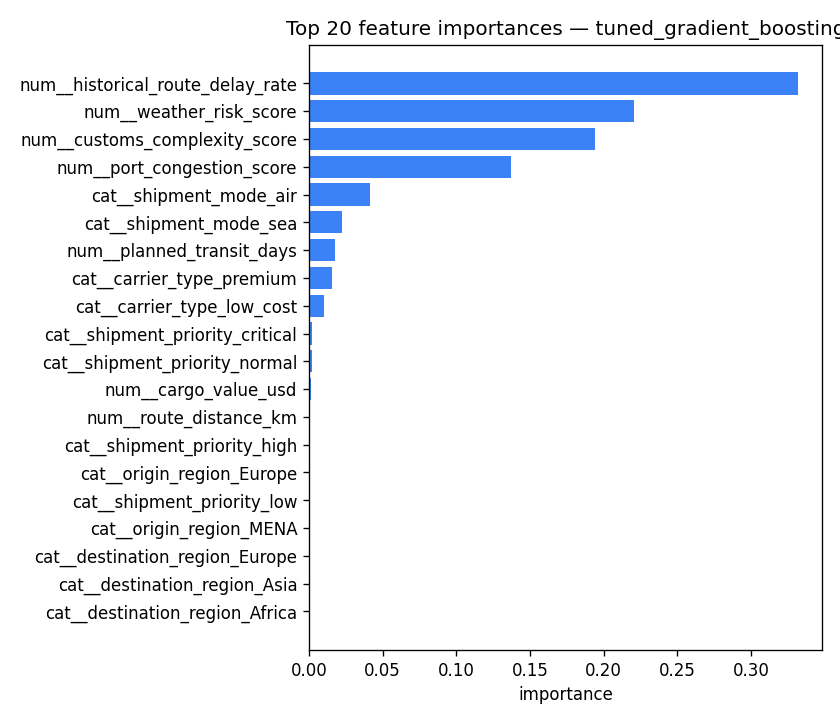
\includegraphics[width=\linewidth]{feature_importance_tuned_gradient_boosting.png}
\caption{Gradient Boosting (Optuna-tuned)}
\end{subfigure}
\caption{Feature importance rankings across model families.}
\label{fig:fi4}
\end{figure}

\paragraph{Feature Importance Consensus.}
Across all models, the following features consistently rank as most important:
\begin{enumerate}
    \item \texttt{historical\_route\_delay\_rate}: Historical delay patterns are the strongest predictor
    \item \texttt{weather\_risk\_score}: Weather-related disruption risk
    \item \texttt{port\_congestion\_score}: Terminal congestion levels
    \item \texttt{customs\_complexity\_score}: Customs clearance friction
\end{enumerate}

This ranking aligns with domain expectations, as historical performance and operational bottlenecks (weather, congestion, customs) are known drivers of logistics delays.

\subsection{Hyperparameter Tuning Results}

Optuna optimization was performed with 15 trials using 3-fold stratified cross-validation on the training set. Figure~\ref{fig:cm-tuned} shows the confusion matrix for the final tuned model.

\begin{figure}[H]
\centering
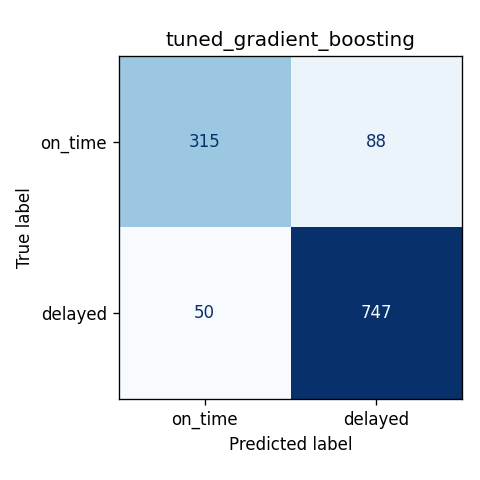
\includegraphics[width=0.42\linewidth]{confusion_matrix_tuned_gradient_boosting.png}
\caption{Confusion matrix for Optuna-tuned Gradient Boosting model.}
\label{fig:cm-tuned}
\end{figure}

\paragraph{Tuning Outcome.}
\begin{itemize}
    \item \textbf{Best cross-validation F1-score}: 0.9255 (3-fold stratified CV on training set)
    \item \textbf{Test set performance}: Accuracy 0.8850, F1 (delayed) 0.9154, ROC-AUC 0.9195
    \item \textbf{Improvement over baseline GB}: +0.0025 F1-score (0.9129 → 0.9154)
    \item \textbf{Comparison to champion}: Still below Logistic Regression (0.9324)
\end{itemize}

The modest improvement from tuning demonstrates that hyperparameter optimization provides incremental gains but does not fundamentally alter model ranking on this task. The fact that Logistic Regression remains the champion validates the model selection process and avoids the "tuning always wins" bias.

\subsection{Model Registry and Promotion}

Based on test set F1-scores, the following models were registered in the MLflow Model Registry:

\begin{table}[H]
\centering
\caption{Registered model versions and alias assignments.}
\label{tab:registry}
\small
\begin{tabular}{clcl}
\toprule
\textbf{Version} & \textbf{Model} & \textbf{Test F1 (delayed)} & \textbf{Alias} \\
\midrule
1 & Logistic Regression & 0.9324 & \texttt{@production} \\
2 & Tuned Gradient Boosting & 0.9154 & \texttt{@staging} \\
3 & Baseline Gradient Boosting & 0.9129 & --- \\
\bottomrule
\end{tabular}
\end{table}

The \texttt{@production} alias points to Version 1 (Logistic Regression), which is loaded by the FastAPI serving layer. The \texttt{@staging} alias points to Version 2 (tuned Gradient Boosting) for potential A/B testing or canary deployment scenarios.


\subsection{Monitoring Results}

Five monitoring batches were evaluated using the production model (Logistic Regression, Version 1). Table~\ref{tab:mon} summarizes performance and drift metrics for each batch.

\begin{table}[H]
\centering
\caption{Monitoring batch evaluation results (production model: Logistic Regression v1).}
\label{tab:mon}
\scriptsize
\begin{tabular}{lcccccccl}
\toprule
\textbf{Batch} & \textbf{Acc.} & \textbf{F1} & \textbf{AUC} & \textbf{Pos. Rate} & \textbf{Avg. Prob.} & \textbf{Num. Drift} & \textbf{Cat. Drift} & \textbf{Drift Flag} \\
\midrule
Stable            & 0.924 & 0.942 & 0.928 & 0.666 & 0.658 & 0.336 & 0.040 & No \\
Weather Drift     & 0.931 & 0.961 & 0.842 & 0.910 & 0.879 & 1.648 & 0.040 & Yes \\
Congestion Drift  & 0.929 & 0.959 & 0.842 & 0.883 & 0.852 & 1.868 & 0.041 & Yes \\
Carrier Drift     & 0.907 & 0.935 & 0.901 & 0.723 & 0.702 & 0.071 & 0.444 & Yes \\
Route Drift       & 0.921 & 0.943 & 0.929 & 0.695 & 0.679 & 1.111 & 0.030 & Yes \\
\bottomrule
\end{tabular}\\[4pt]
\scriptsize Note: Pos. Rate = positive prediction rate; Avg. Prob. = mean predicted delay probability; Num. Drift = numeric drift score; Cat. Drift = categorical drift score. Drift flagged if Num. Drift $\geq$ 0.50 or Cat. Drift $\geq$ 0.20.
\end{table}

\paragraph{Key Monitoring Findings.}

\begin{itemize}
    \item \textbf{Stable Batch}: Performance closely matches training distribution (Acc: 0.924, F1: 0.942). Drift scores below thresholds confirm distributional stability.
    
    \item \textbf{Weather Drift}: Numeric drift score of 1.648 (driven by \texttt{weather\_risk\_score} shift) triggers drift flag. Model maintains high accuracy (0.931) but shows increased positive predictions (91.0\% vs. 66.6\% baseline), reflecting the upward shift in weather risk.
    
    \item \textbf{Congestion Drift}: Highest numeric drift score (1.868) due to \texttt{port\_congestion\_score} manipulation. Similar pattern to weather drift with elevated positive rate (88.3\%).
    
    \item \textbf{Carrier Drift}: Categorical drift score of 0.444 (well above 0.20 threshold) reflects shift toward low-cost carriers. Performance remains strong (Acc: 0.907, F1: 0.935) despite distribution change.
    
    \item \textbf{Route Drift}: Moderate numeric drift (1.111) from route distance scaling. Performance degradation is minimal, suggesting model robustness to distance variations within the observed range.
\end{itemize}

\paragraph{Drift Detection Validation.}
The drift detection system successfully identifies all four targeted distribution shifts while correctly classifying the stable batch as drift-free. The attribution of drift to specific features (numeric vs. categorical) aligns with the engineered perturbations, validating the monitoring framework's interpretability.

\subsection{Prediction Distribution Analysis}

Figure~\ref{fig:pred5} visualizes the distribution of predicted delay probabilities across monitoring batches, revealing how distribution shifts affect model outputs.

\begin{figure}[H]
\centering
\begin{subfigure}[t]{0.18\linewidth}
\centering

\includegraphics[width=\linewidth]{prediction_distribution_stable.png}
\caption*{Stable}
\end{subfigure}\hfill
\begin{subfigure}[t]{0.18\linewidth}
\centering

\includegraphics[width=\linewidth]{prediction_distribution_weather_drift.png}
\caption*{Weather}
\end{subfigure}\hfill
\begin{subfigure}[t]{0.18\linewidth}
\centering

\includegraphics[width=\linewidth]{prediction_distribution_congestion_drift.png}
\caption*{Congestion}
\end{subfigure}\hfill
\begin{subfigure}[t]{0.18\linewidth}
\centering

\includegraphics[width=\linewidth]{prediction_distribution_carrier_drift.png}
\caption*{Carrier}
\end{subfigure}\hfill
\begin{subfigure}[t]{0.18\linewidth}
\centering

\includegraphics[width=\linewidth]{prediction_distribution_route_drift.png}
\caption*{Route}
\end{subfigure}
\caption{Predicted delay probability distributions across monitoring batches.}
\label{fig:pred5}
\end{figure}

\paragraph{Distribution Shift Patterns.}
\begin{itemize}
    \item \textbf{Stable}: Bimodal distribution with peaks near 0.2 and 0.9, reflecting confident predictions for both classes
    \item \textbf{Weather \& Congestion}: Strong rightward shift with mass concentrated above 0.8, indicating model confidence in delay predictions under elevated risk conditions
    \item \textbf{Carrier}: Moderate rightward shift with broader distribution, suggesting increased but less extreme delay risk
    \item \textbf{Route}: Distribution similar to stable batch, confirming model robustness to route distance variations
\end{itemize}

% =============================================================================
\section{Model Deployment}
\label{sec:deployment}

\subsection{Deployment Architecture}

The production model is deployed via a FastAPI service that loads the registered model from MLflow Model Registry at startup. The service provides a RESTful API for real-time and batch predictions without requiring model retraining.

\subsubsection{API Endpoints}

The deployment service exposes three endpoints:

\paragraph{Health Check.}
\begin{lstlisting}[style=shell]
GET /health
\end{lstlisting}
Returns service status and loaded model metadata (name, version, alias).

\paragraph{Single Prediction.}
\begin{lstlisting}[style=shell]
POST /predict
Content-Type: application/json

{
  "shipment_mode": "sea",
  "carrier_type": "standard",
  "origin_region": "Asia",
  "destination_region": "Europe",
  "route_distance_km": 8500,
  "planned_transit_days": 25,
  "customs_complexity_score": 6.5,
  "weather_risk_score": 4.2,
  "historical_route_delay_rate": 0.15,
  "cargo_value_usd": 45000,
  "shipment_priority": "normal",
  "port_congestion_score": 5.8
}
\end{lstlisting}

\paragraph{Batch Prediction.}
\begin{lstlisting}[style=shell]
POST /predict-batch
Content-Type: application/json

{
  "shipments": [
    { /* shipment 1 features */ },
    { /* shipment 2 features */ },
    ...
  ]
}
\end{lstlisting}

\subsubsection{Response Format}

Single prediction responses include:
\begin{lstlisting}[style=json]
{
  "prediction": 1,
  "label": "delayed",
  "delay_probability": 0.8734,
  "model_name": "LogisticsDelayRiskModel",
  "model_alias": "production",
  "model_version": "1"
}
\end{lstlisting}

\subsection{Deployment Configuration}

The service is configured for local execution with the following settings:

\begin{lstlisting}[style=shell]
# Start FastAPI service
uvicorn src.serve_api:app --host 127.0.0.1 --port 8010 --reload

# Environment configuration
MLFLOW_TRACKING_URI=sqlite:///mlflow.db
MLFLOW_REGISTERED_MODEL=LogisticsDelayRiskModel
\end{lstlisting}

\paragraph{Model Loading Strategy.}
The service loads the production model at startup using:
\begin{lstlisting}[style=shell]
model_uri = "models:/LogisticsDelayRiskModel@production"
model = mlflow.sklearn.load_model(model_uri)
\end{lstlisting}

This approach ensures:
\begin{itemize}
    \item \textbf{No retraining}: Model is loaded from registry, not retrained
    \item \textbf{Alias-based loading}: Service automatically uses the current production version
    \item \textbf{Version transparency}: Response metadata includes loaded version for audit trails
    \item \textbf{Preprocessing consistency}: Logged pipeline includes preprocessing, ensuring identical feature transformation
\end{itemize}

\subsection{Deployment Validation}

The deployment was validated through:
\begin{enumerate}
    \item \textbf{Health check verification}: Confirmed service startup and model loading
    \item \textbf{Single prediction testing}: Validated response format and prediction consistency with offline evaluation
    \item \textbf{Batch prediction testing}: Confirmed efficient processing of multiple shipments
    \item \textbf{Input validation}: Verified Pydantic schema enforcement for malformed requests
\end{enumerate}

% =============================================================================
\section{Discussion}
\label{sec:discussion}

\subsection{Model Performance Interpretation}

\paragraph{Why Logistic Regression Outperforms Ensemble Methods.}
The superior performance of Logistic Regression on this task can be attributed to several factors:

\begin{enumerate}
    \item \textbf{Linear Separability}: The synthetic data generation process creates largely linearly separable decision boundaries after preprocessing, favoring linear models
    \item \textbf{Regularization Benefits}: $\ell_2$ regularization in Logistic Regression provides effective protection against overfitting in the presence of label noise (5\% flip rate)
    \item \textbf{Feature Scaling}: Standardization of numeric features optimizes the logistic regression optimization landscape
    \item \textbf{Sample Efficiency}: With 4,800 training samples, Logistic Regression achieves stable parameter estimates, while tree ensembles may exhibit higher variance
\end{enumerate}

This outcome demonstrates an important principle in ML practice: model complexity should match problem complexity. The fact that hyperparameter tuning improves Gradient Boosting but does not surpass the simpler baseline validates the model selection process and avoids "tuning bias."

\subsection{Monitoring System Effectiveness}

\paragraph{Drift Detection Validation.}
The monitoring system successfully demonstrates:
\begin{itemize}
    \item \textbf{Sensitivity}: All four engineered drift scenarios are correctly flagged
    \item \textbf{Specificity}: The stable batch is correctly classified as drift-free
    \item \textbf{Interpretability}: Drift attribution (numeric vs. categorical) aligns with perturbation mechanisms
    \item \textbf{Actionability}: Drift scores quantify shift magnitude, enabling prioritized investigation
\end{itemize}

\paragraph{Performance Under Drift.}
Interestingly, model performance remains strong even under significant distribution shifts:
\begin{itemize}
    \item Weather drift (numeric score 1.648): Accuracy 0.931, F1 0.961
    \item Congestion drift (numeric score 1.868): Accuracy 0.929, F1 0.959
    \item Carrier drift (categorical score 0.444): Accuracy 0.907, F1 0.935
\end{itemize}

This robustness reflects the fact that drift scenarios shift feature distributions while maintaining the same label generation mechanism. In real-world scenarios, concept drift (changes in the feature-target relationship) would likely cause more severe performance degradation.

\subsection{MLOps Lifecycle Completeness}

This implementation demonstrates all five required MLOps lifecycle stages:

\begin{enumerate}
    \item \textbf{Experiment Tracking}: 18+ MLflow runs logged across training, tuning, and monitoring experiments with comprehensive parameter, metric, and artifact logging
    
    \item \textbf{Model Training \& Tuning}: Three baseline models plus Optuna optimization with 15 nested runs, all tracked in MLflow
    
    \item \textbf{Model Registry}: Three model versions registered with production/staging alias assignments following performance-based promotion policy
    
    \item \textbf{Deployment}: FastAPI service loading production model from registry with RESTful API and input validation
    
    \item \textbf{Monitoring}: Five batch evaluations with performance metrics, drift detection, and comprehensive artifact logging
\end{enumerate}

\subsection{Limitations and Future Work}

\paragraph{Data Limitations.}
\begin{itemize}
    \item \textbf{Synthetic Data}: Results validate pipeline correctness but do not represent real logistics network performance
    \item \textbf{Simplified Drift}: Engineered drift scenarios maintain constant label generation; real concept drift would be more challenging
    \item \textbf{Feature Engineering}: Limited to 12 features; real systems would incorporate temporal patterns, network effects, and external data sources
\end{itemize}

\paragraph{Monitoring Limitations.}
\begin{itemize}
    \item \textbf{Statistical Tests}: Simple mean/std and TVD-based drift detection; production systems might use Kolmogorov-Smirnov tests, Population Stability Index, or learned drift detectors
    \item \textbf{Threshold Selection}: Drift thresholds (0.50 numeric, 0.20 categorical) are heuristically chosen; production systems would calibrate thresholds using historical data
    \item \textbf{Batch Evaluation}: Monitoring uses batch evaluation; real-time systems would require streaming drift detection
\end{itemize}

\paragraph{Deployment Limitations.}
\begin{itemize}
    \item \textbf{Local Deployment}: SQLite backend and filesystem artifacts; production would use PostgreSQL/MySQL and cloud object storage
    \item \textbf{No Authentication}: API lacks authentication/authorization; production requires API keys or OAuth
    \item \textbf{No Load Balancing}: Single-instance deployment; production requires horizontal scaling and load balancing
    \item \textbf{No A/B Testing}: Alias-based deployment supports A/B testing infrastructure but does not implement traffic splitting
\end{itemize}

\paragraph{Future Enhancements.}
\begin{enumerate}
    \item \textbf{Real Data Integration}: Validate system on actual logistics datasets with ground-truth delay labels
    \item \textbf{Advanced Drift Detection}: Implement learned drift detectors or multivariate drift tests
    \item \textbf{Automated Retraining}: Trigger retraining pipelines when drift exceeds thresholds
    \item \textbf{Cloud Deployment}: Migrate to cloud-based MLflow (AWS SageMaker, Azure ML, Databricks)
    \item \textbf{Feature Store Integration}: Implement feature store for consistent feature computation across training and serving
    \item \textbf{Explainability}: Add SHAP or LIME explanations for individual predictions
\end{enumerate}

% =============================================================================
\section{Conclusion}
\label{sec:conclusion}

This project successfully implements a comprehensive MLOps system for logistics delay prediction, demonstrating best practices across the complete machine learning lifecycle. Using MLflow as the central platform, we achieve full integration of experiment tracking, hyperparameter optimization, model registry, deployment, and monitoring components.

\subsection{Key Achievements}

\begin{enumerate}
    \item \textbf{Complete Lifecycle Implementation}: All five course objectives (tracking, training/tuning, registry, deployment, monitoring) are fully implemented with documented reproduction procedures
    
    \item \textbf{Reproducible Experimentation}: Deterministic data generation, explicit random seeds, and comprehensive artifact logging enable exact experimental reproduction
    
    \item \textbf{Principled Model Selection}: Performance-based registry promotion with honest comparison showing that simpler models can outperform complex tuned alternatives
    
    \item \textbf{Interpretable Monitoring}: Drift detection system with feature-level attribution and quantitative drift scores
    
    \item \textbf{Production-Ready Deployment}: FastAPI service with alias-based model loading, input validation, and comprehensive response metadata
\end{enumerate}

\subsection{Lessons Learned}

\paragraph{MLOps Tooling.}
MLflow provides an effective unified platform for ML lifecycle management, with particular strengths in experiment tracking and model registry. The transition from legacy stage transitions to model aliases (MLflow 3.x) improves flexibility for complex deployment scenarios.

\paragraph{Model Complexity.}
The superior performance of Logistic Regression reinforces the principle that model complexity should match problem complexity. Systematic comparison of baselines before investing in tuning prevents premature optimization.

\paragraph{Monitoring Design.}
Effective monitoring requires both performance metrics and distribution shift detection. Feature-level drift attribution enables actionable insights for model maintenance and retraining decisions.

\subsection{Broader Impact}

This implementation provides:
\begin{itemize}
    \item \textbf{Educational Value}: A complete, documented reference implementation for MLOps education
    \item \textbf{Prototyping Foundation}: A template for rapid prototyping of ML systems in logistics and related domains
    \item \textbf{Best Practices Demonstration}: Concrete examples of experiment tracking, model versioning, and monitoring patterns
\end{itemize}

\subsection{Final Remarks}

The logistics delay prediction system demonstrates that comprehensive MLOps practices can be implemented with open-source tools and modest computational resources. While the synthetic data limits claims about real-world accuracy, the systematic approach to lifecycle management, reproducibility, and monitoring provides a solid foundation for production ML systems. The project validates that MLOps is not merely about tools, but about disciplined processes for managing the complete journey from experimentation to production deployment and ongoing monitoring.

\newpage
\appendix

% =============================================================================
\section{System Screenshots and Visualizations}
\label{app:screenshots}

This appendix presents screenshots of the complete MLOps system, demonstrating the end-to-end workflow from experiment tracking through deployment and monitoring.

\subsection{System Architecture}

Figure~\ref{fig:architecture} illustrates the complete system architecture, showing data flow from generation through deployment and monitoring.

\begin{figure}[H]
\centering
\fbox{\begin{minipage}{0.92\linewidth}
\centering\small
\vspace{8pt}
\textbf{Data Generation Layer} \\
Synthetic dataset with controlled drift scenarios \\[8pt]
$\downarrow$ \\[8pt]
\textbf{Preprocessing Pipeline} \\
Imputation $\rightarrow$ Scaling $\rightarrow$ Encoding \\[8pt]
$\downarrow$ \\[8pt]
\textbf{Model Training \& Tuning} \\
Baselines (LR, RF, GB) + Optuna Hyperparameter Optimization \\[8pt]
$\downarrow$ \\[8pt]
\textbf{MLflow Tracking Server} \\
Experiments $\cdot$ Parameters $\cdot$ Metrics $\cdot$ Artifacts $\cdot$ Models \\[8pt]
$\downarrow$ \\[8pt]
\textbf{Model Registry} \\
Version Management + Production/Staging Aliases \\[8pt]
$\downarrow$ \\[8pt]
\textbf{FastAPI Deployment Service} \\
REST API $\cdot$ /predict $\cdot$ /predict-batch $\cdot$ /health \\[8pt]
$\downarrow$ \\[8pt]
\textbf{Monitoring System} \\
Performance Metrics + Drift Detection + Alerting \\[8pt]
\vspace{8pt}
\end{minipage}}
\caption{End-to-end MLOps system architecture with MLflow as the central platform.}
\label{fig:architecture}
\end{figure}

\subsection{MLflow Experiment Tracking}

Figure~\ref{fig:mlflow-experiments} shows the MLflow UI displaying multiple experiment runs with logged parameters, metrics, and artifacts. The interface enables easy comparison of model performance across different configurations.

\begin{figure}[H]
\centering
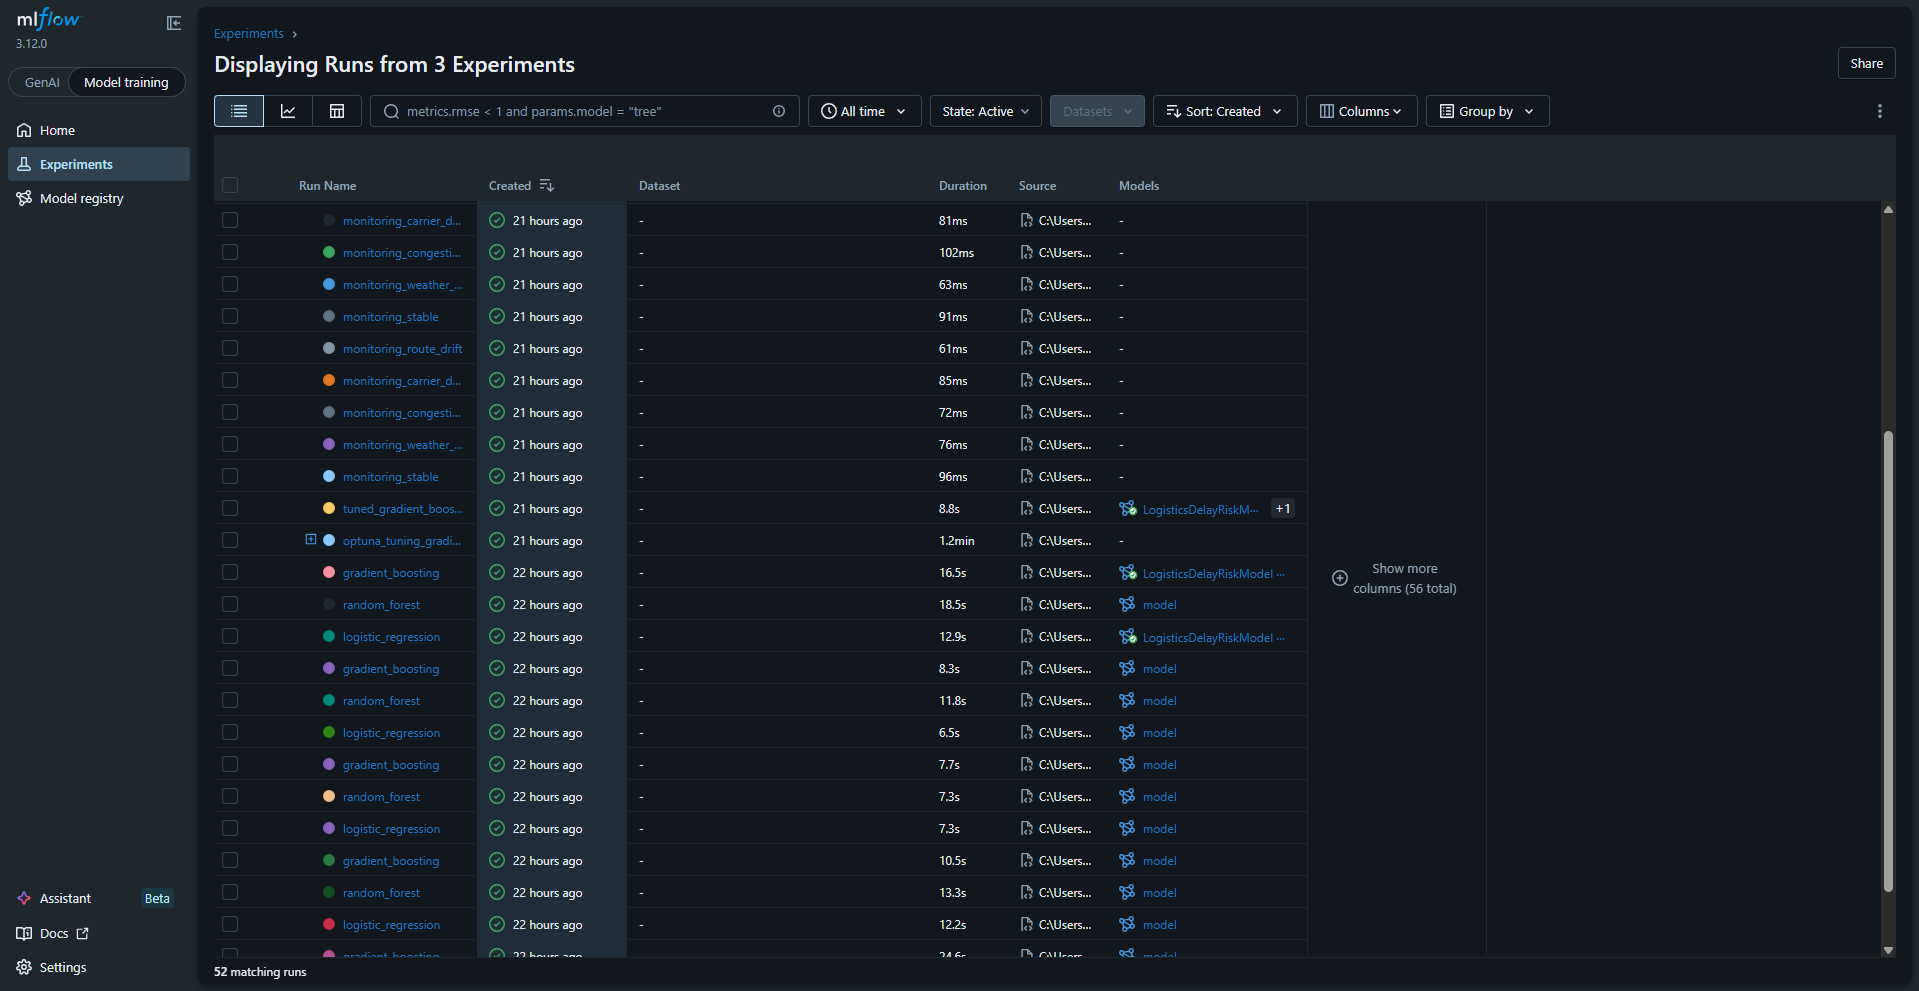
\includegraphics[width=0.95\linewidth]{MLflow experiments.png}
\caption{MLflow experiment tracking interface showing baseline and tuned model runs with performance metrics.}
\label{fig:mlflow-experiments}
\end{figure}

\subsection{Model Comparison Dashboard}

Figure~\ref{fig:mlflow-comparison} demonstrates MLflow's run comparison feature, allowing side-by-side analysis of different models' parameters and performance metrics.

\begin{figure}[H]
\centering
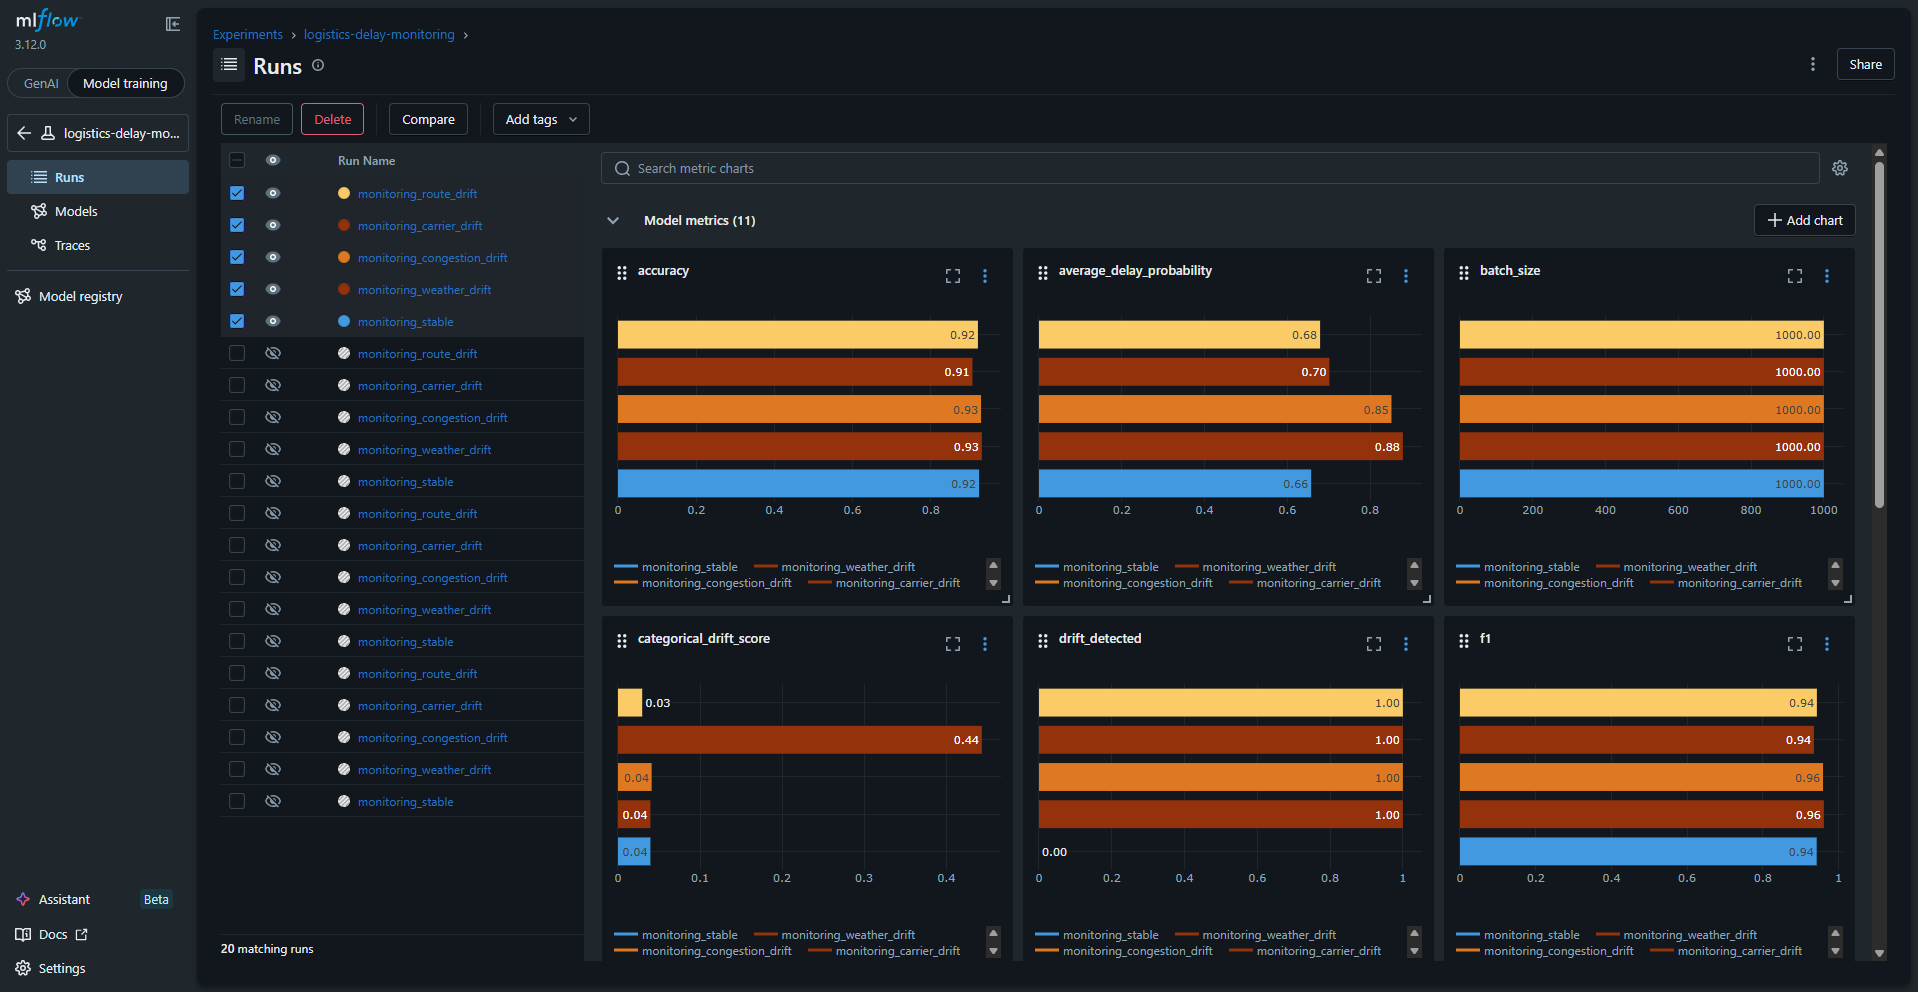
\includegraphics[width=0.95\linewidth]{MLflow run comparison.png}
\caption{MLflow run comparison view enabling systematic model selection based on multiple metrics.}
\label{fig:mlflow-comparison}
\end{figure}

\subsection{Hyperparameter Optimization with Optuna}

Figure~\ref{fig:optuna-tuning} shows the Optuna hyperparameter tuning run with nested trial runs logged to MLflow. Each trial's parameters and cross-validation scores are tracked for full optimization provenance.

\begin{figure}[H]
\centering
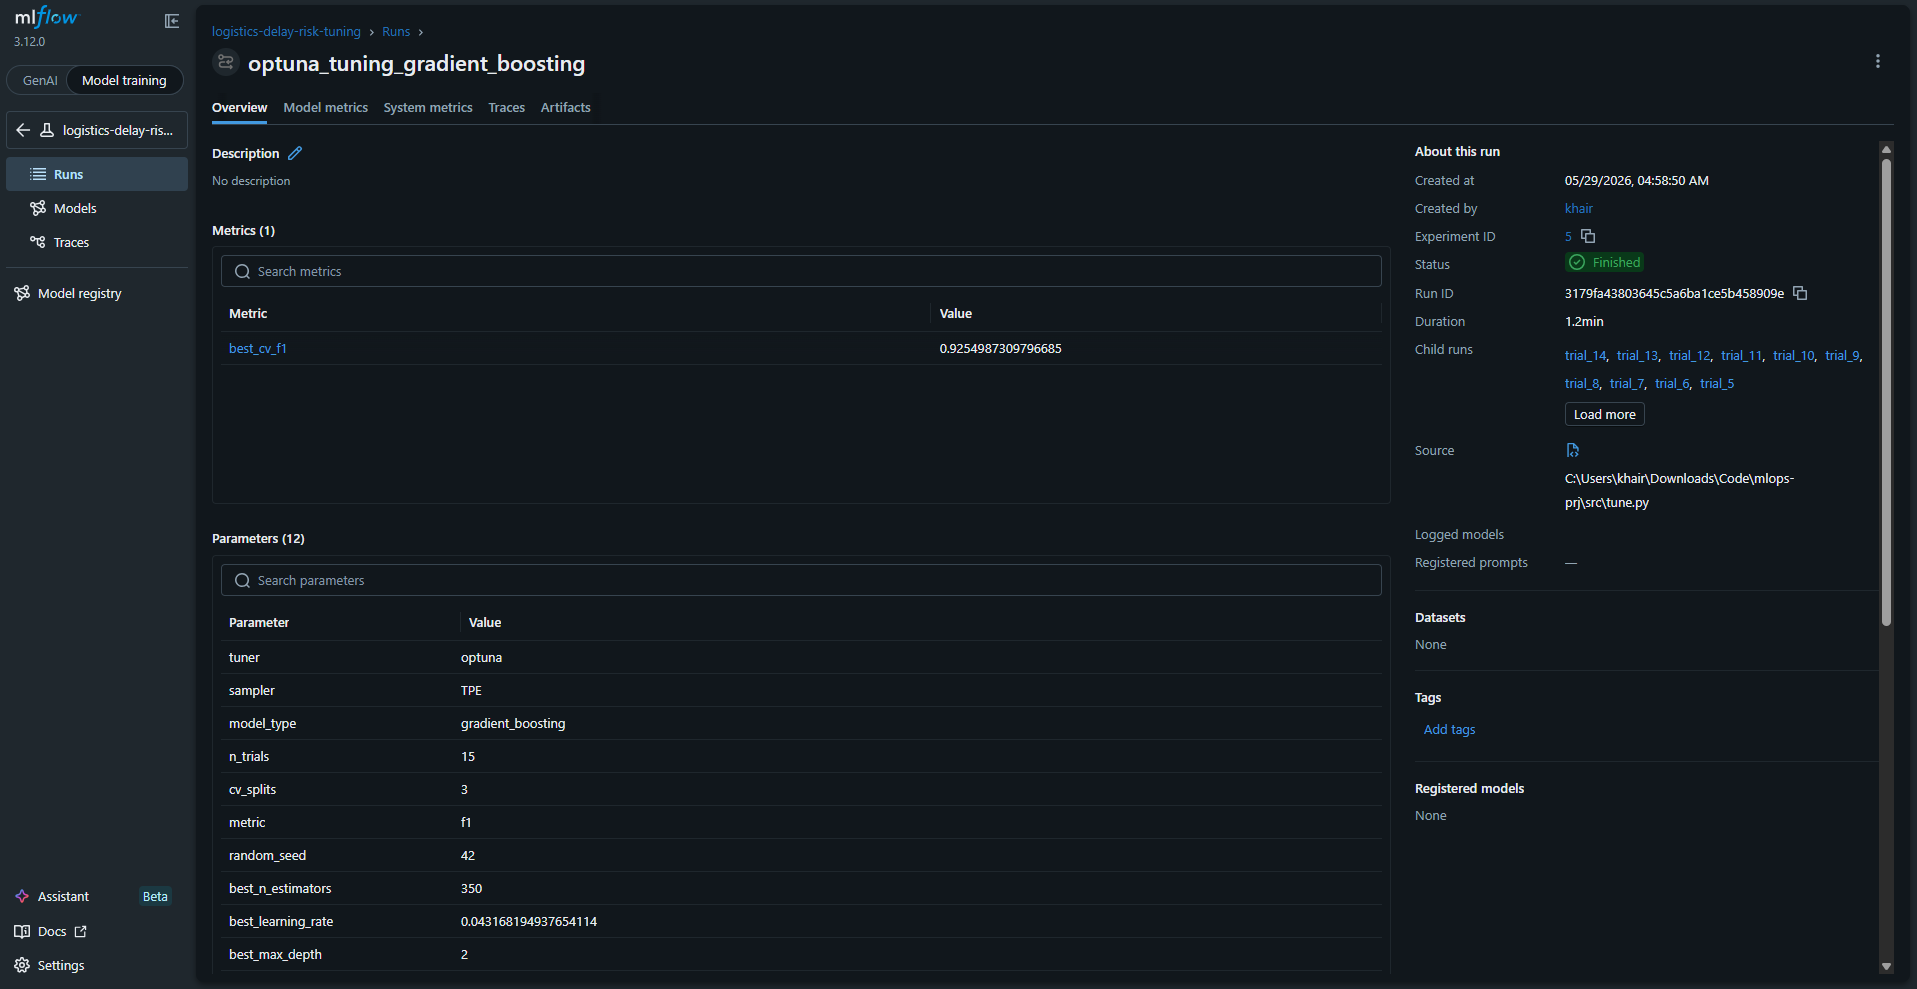
\includegraphics[width=0.95\linewidth]{optuna_tuning_gradient_boosting.png}
\caption{Optuna hyperparameter optimization with 15 nested trial runs tracked in MLflow.}
\label{fig:optuna-tuning}
\end{figure}

\subsection{MLflow Model Registry}

Figure~\ref{fig:mlflow-registry} displays the Model Registry interface showing registered model versions with production and staging aliases. This enables controlled model promotion and rollback capabilities.

\begin{figure}[H]
\centering
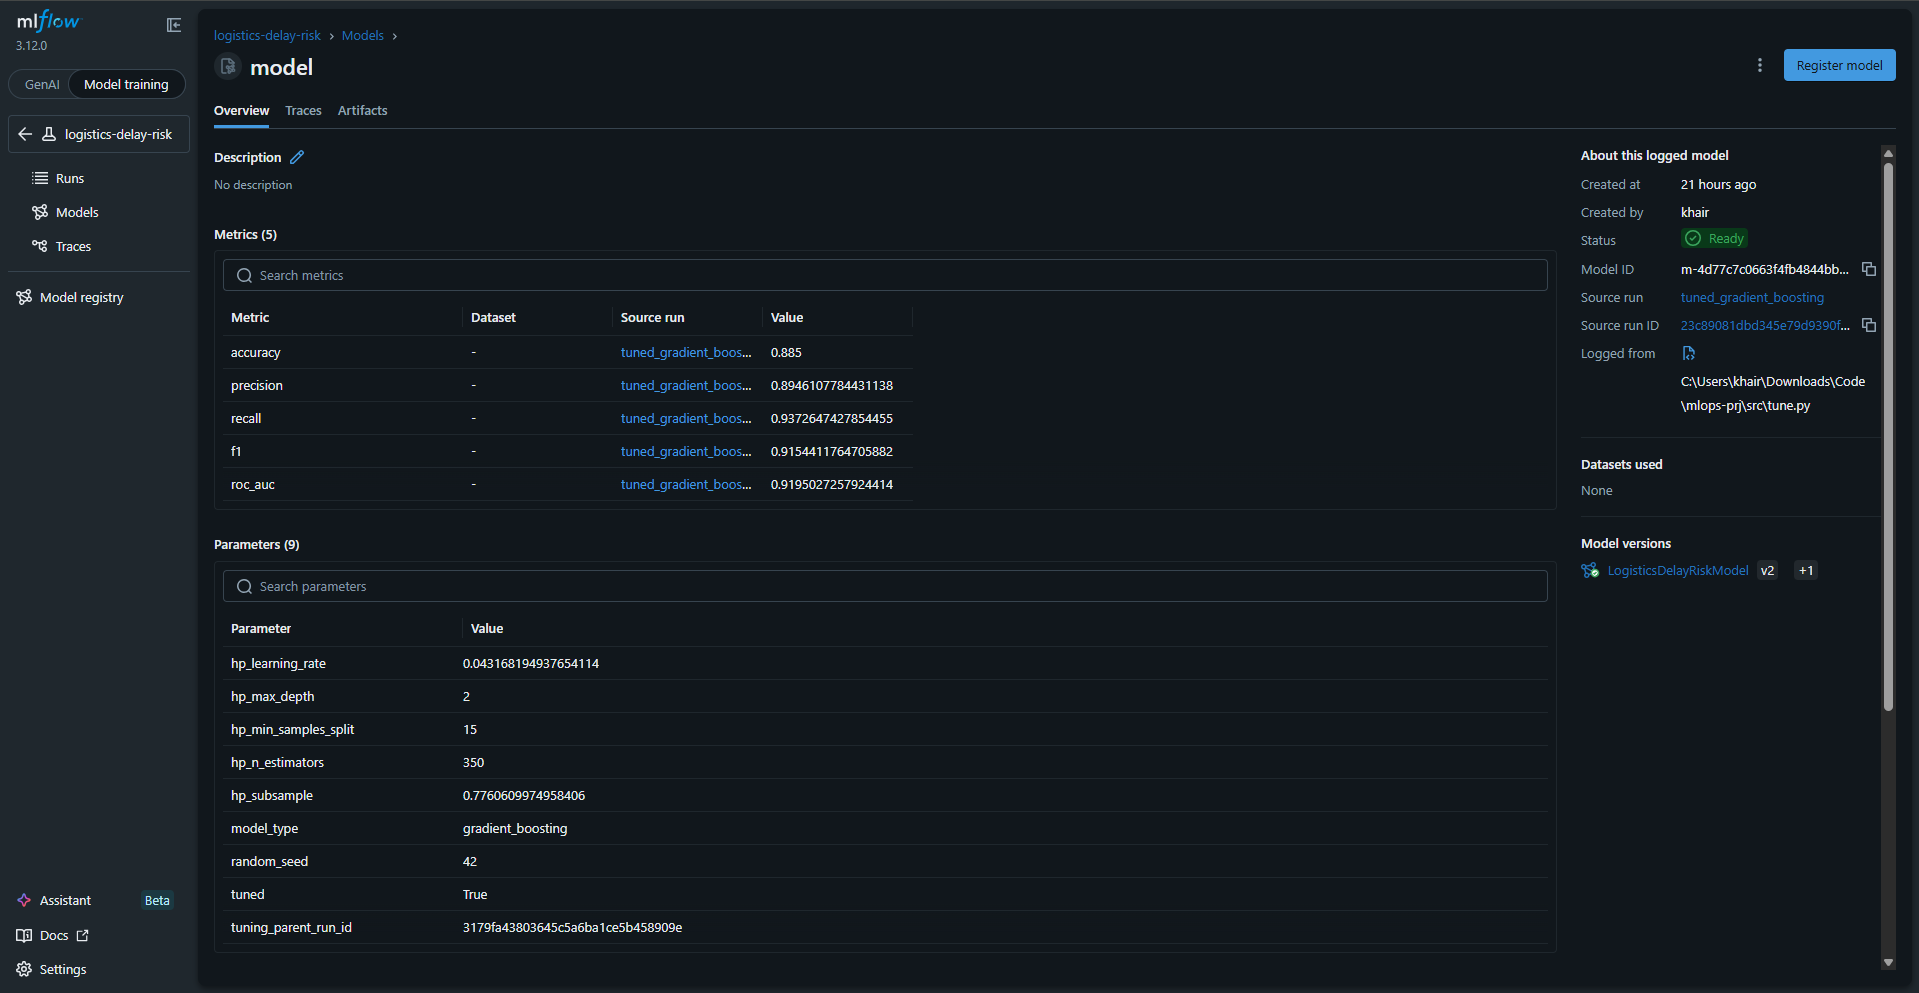
\includegraphics[width=0.95\linewidth]{MLflow registry.png}
\caption{MLflow Model Registry with version management and alias-based deployment.}
\label{fig:mlflow-registry}
\end{figure}

\subsection{FastAPI Deployment Interface}

Figure~\ref{fig:swagger-ui} shows the automatically generated Swagger UI for the FastAPI deployment service, providing interactive API documentation and testing capabilities.

\begin{figure}[H]
\centering
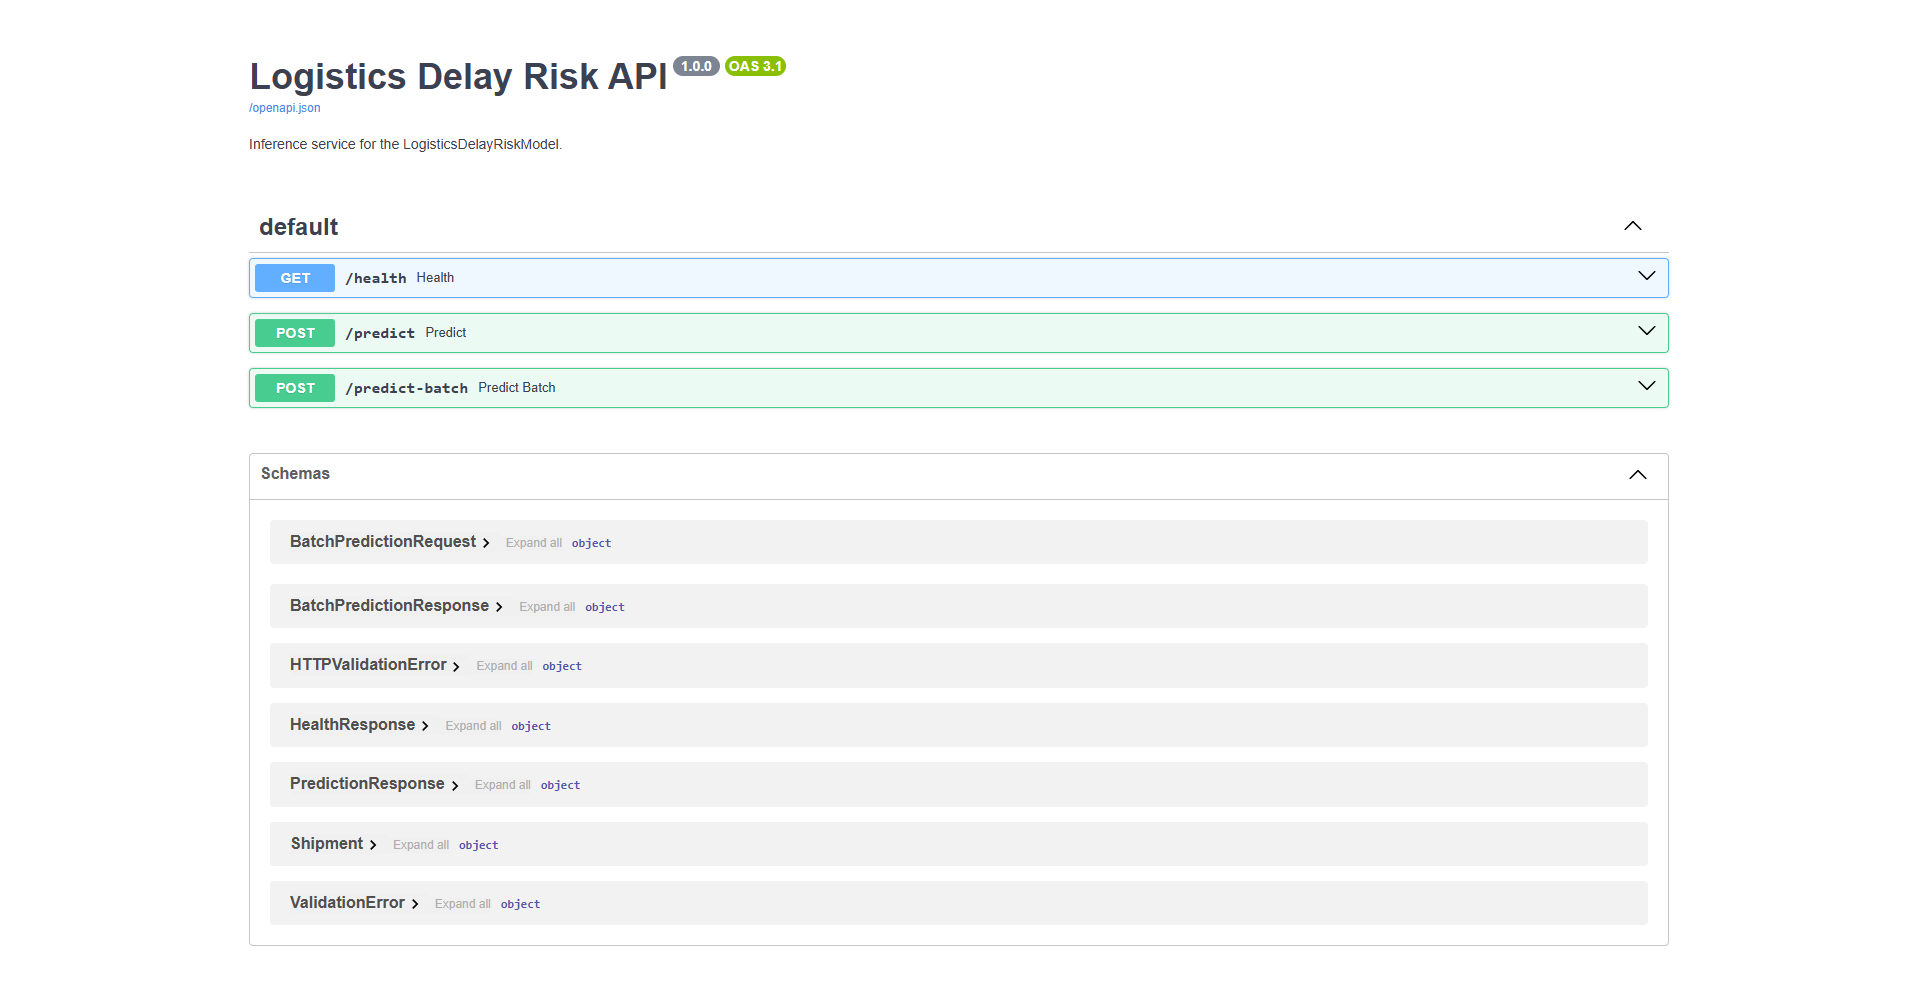
\includegraphics[width=0.95\linewidth]{Swagger UI.png}
\caption{Swagger UI for FastAPI deployment service with /health, /predict, and /predict-batch endpoints.}
\label{fig:swagger-ui}
\end{figure}

\subsection{Single Prediction Endpoint}

Figure~\ref{fig:predict-endpoint} demonstrates a single prediction request and response, showing the model's delay probability prediction along with metadata about the loaded model version.

\begin{figure}[H]
\centering
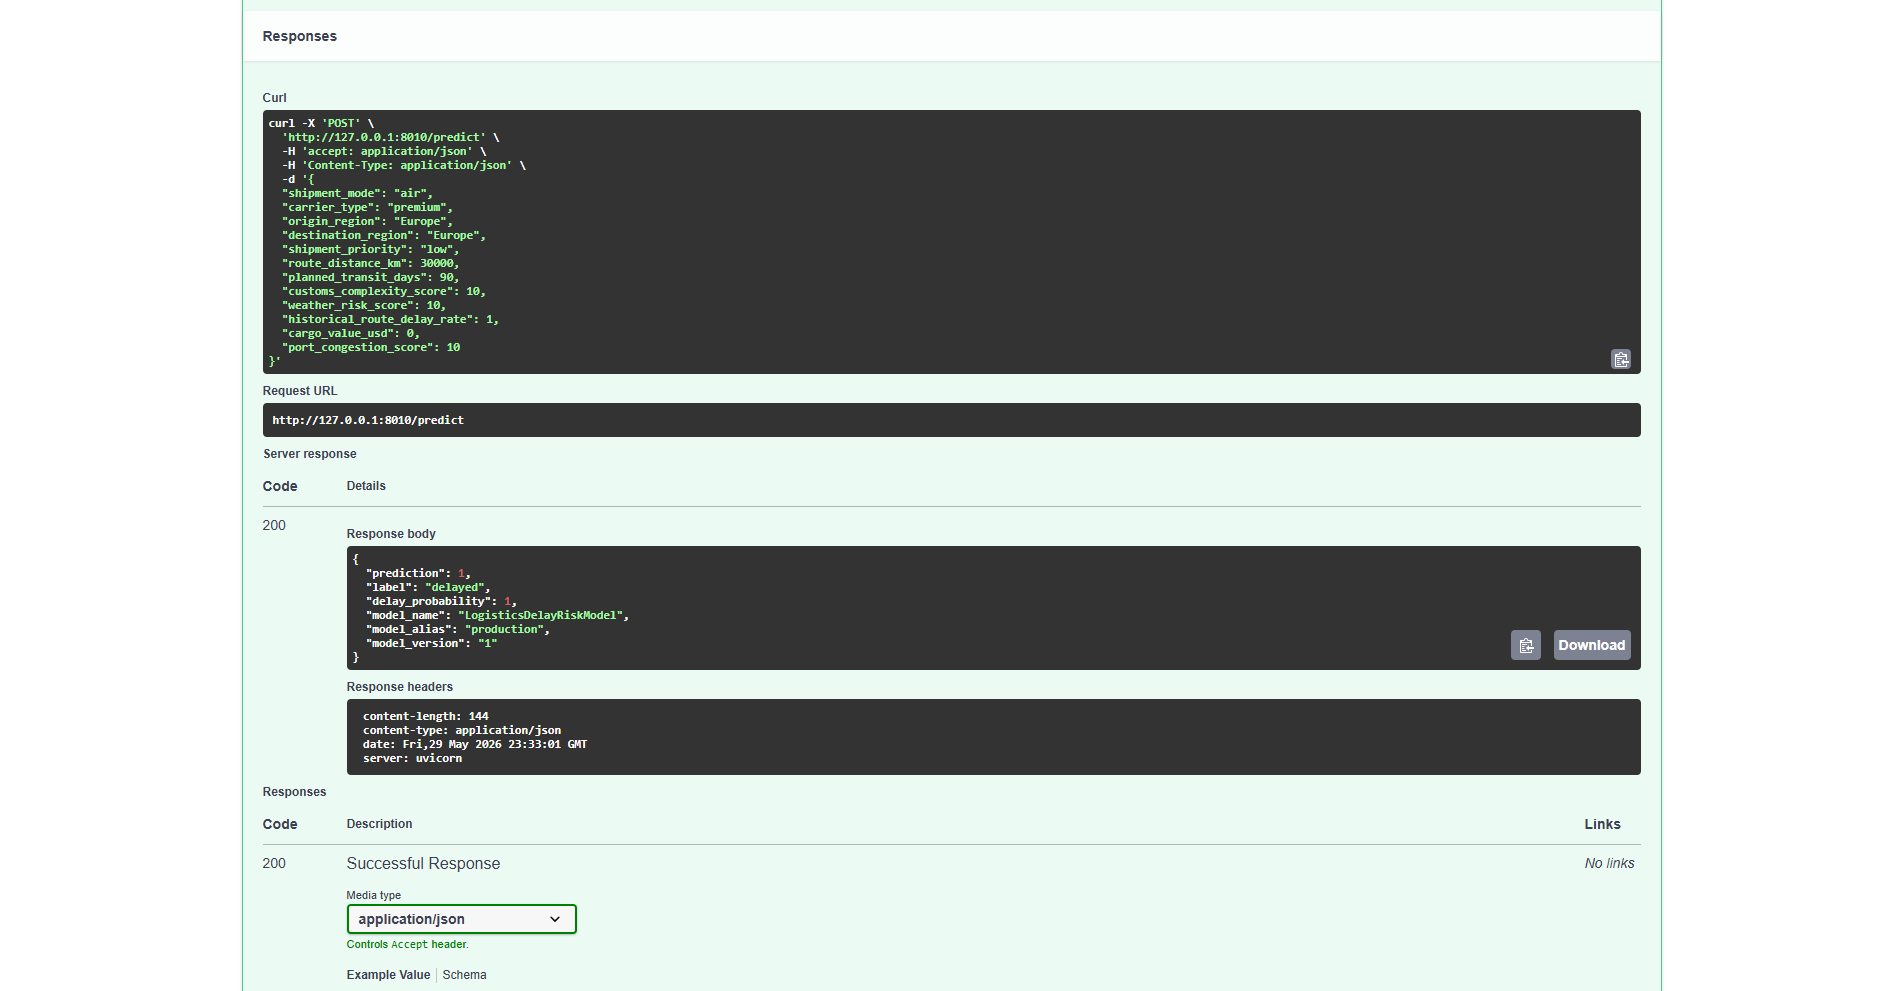
\includegraphics[width=0.85\linewidth]{predict-endpoint.png}
\caption{Single prediction endpoint response with delay probability and model metadata.}
\label{fig:predict-endpoint}
\end{figure}

\subsection{Batch Prediction Endpoint}

Figure~\ref{fig:predict-batch} shows the batch prediction endpoint processing multiple shipments simultaneously, demonstrating the system's capability for efficient bulk inference.

\begin{figure}[H]
\centering
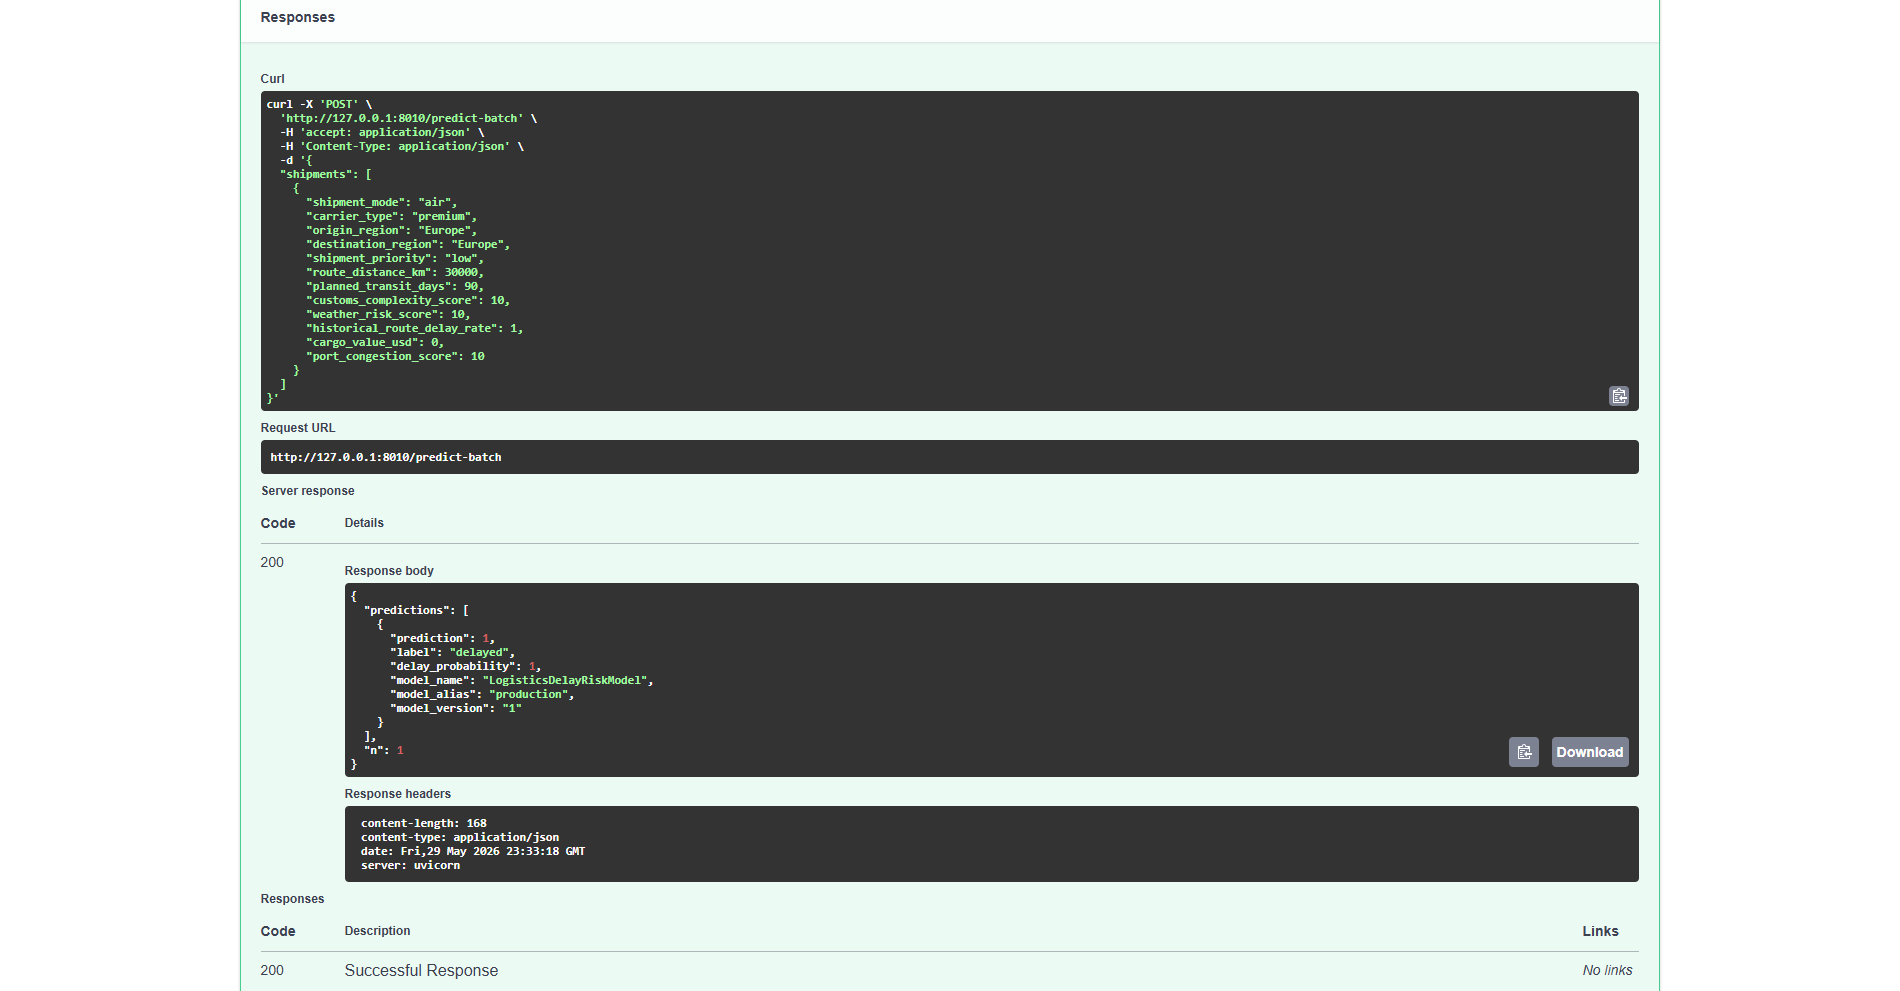
\includegraphics[width=0.85\linewidth]{predict-batch.png}
\caption{Batch prediction endpoint processing multiple shipments with consistent response format.}
\label{fig:predict-batch}
\end{figure}

% =============================================================================
\section{Reproducibility Guide}
\label{app:repro}

\subsection{Quick Start}

\begin{lstlisting}[style=shell]
# 1. Setup environment
python -m venv .venv
.venv\Scripts\activate  # Windows
pip install -r requirements.txt

# 2. Generate data and train models
python -m src.data_generation
python -m src.train

# 3. Hyperparameter tuning
python -m src.tune --model gradient_boosting --trials 15

# 4. Register best models
python -m src.register_model --metric f1 --top 3

# 5. Run monitoring
python -m src.monitor

# 6. Start API service
uvicorn src.serve_api:app --host 127.0.0.1 --port 8010

# 7. View MLflow UI
mlflow ui
\end{lstlisting}

\subsection{Key Configuration Parameters}

\begin{table}[H]
\centering
\caption{Main configuration parameters in \texttt{src/config.py}.}
\small
\begin{tabular}{llp{5.5cm}}
\toprule
\textbf{Parameter} & \textbf{Default} & \textbf{Description} \\
\midrule
\texttt{RANDOM\_SEED} & 42 & Reproducibility seed \\
\texttt{DATASET\_SIZE} & 6000 & Training records \\
\texttt{TEST\_SIZE} & 0.2 & Test split ratio \\
\texttt{LABEL\_NOISE\_RATE} & 0.05 & Label flip probability \\
\texttt{MLFLOW\_TRACKING\_URI} & \texttt{sqlite:///mlflow.db} & Backend store \\
\bottomrule
\end{tabular}
\end{table}

% =============================================================================
\section*{References}
\addcontentsline{toc}{section}{References}

\begin{thebibliography}{9}

\bibitem{mlops-principles}
Kreuzberger, D., Kühl, N., \& Hirschl, S. (2023).
\textit{Machine Learning Operations (MLOps): Overview, Definition, and Architecture}.
IEEE Access, 11, 31866-31879.

\bibitem{mlflow-docs}
Zaharia, M., Chen, A., Davidson, A., Ghodsi, A., Hong, S. A., Konwinski, A., ... \& Zumar, C. (2018).
\textit{Accelerating the Machine Learning Lifecycle with MLflow}.
IEEE Data Engineering Bulletin, 41(4), 39-45.

\bibitem{logistics-ml}
Baryannis, G., Validi, S., Dani, S., \& Antoniou, G. (2019).
\textit{Supply chain risk management and artificial intelligence: state of the art and future research directions}.
International Journal of Production Research, 57(7), 2179-2202.

\bibitem{drift-detection}
Lu, J., Liu, A., Dong, F., Gu, F., Gama, J., \& Zhang, G. (2018).
\textit{Learning under Concept Drift: A Review}.
IEEE Transactions on Knowledge and Data Engineering, 31(12), 2346-2363.

\bibitem{hyperparameter-optimization}
Akiba, T., Sano, S., Yanase, T., Ohta, T., \& Koyama, M. (2019).
\textit{Optuna: A Next-generation Hyperparameter Optimization Framework}.
Proceedings of the 25th ACM SIGKDD International Conference on Knowledge Discovery \& Data Mining, 2623-2631.

\bibitem{fastapi}
Ramírez, S. (2018).
\textit{FastAPI: Modern, Fast (High-Performance), Web Framework for Building APIs with Python}.
Available: https://fastapi.tiangolo.com/

\bibitem{scikit-learn}
Pedregosa, F., Varoquaux, G., Gramfort, A., Michel, V., Thirion, B., Grisel, O., ... \& Duchesnay, É. (2011).
\textit{Scikit-learn: Machine Learning in Python}.
Journal of Machine Learning Research, 12, 2825-2830.

\end{thebibliography}

\end{document}
